\documentclass[acmsmall,review]{acmart}

% Packages not loaded by acmart
\usepackage{algorithm}
\usepackage{algpseudocode}
\usepackage{multirow}
\usepackage{placeins}
\usepackage{colortbl}

% Custom math commands
\newcommand{\ec}{\text{ec}}
\newcommand{\onevec}{\mathbf{1}}
\newcommand{\Ztwo}{\mathbb{Z}_2}
\newcommand{\bigO}{\mathcal{O}}
\newcommand{\F}{\mathbb{F}_2}
\newcommand{\Z}{\mathbb{Z}}
\newcommand{\C}{\mathbb{C}}
\newcommand{\HomG}{H_1(G; \Ztwo)}
\newcommand{\inner}[2]{\langle #1, #2 \rangle}

\DeclareMathOperator{\Tr}{Tr}

%%% ACM Journal metadata
\acmJournal{JEA}
\setcopyright{none}          % change to acmlicensed for camera-ready

\title{Efficient Implementation of Exact Eulerian Circuit Counting via the Fast Walsh--Hadamard Transform}

\author{[Author Name]}
\email{[email]}
\affiliation{%
  \institution{[Institution]}
  \city{[City]}
  \country{[Country]}
}

\begin{document}

\begin{abstract}
		Counting the number of Eulerian circuits in undirected graphs is a fundamental \#P-complete problem, lacking the elegant determinantal solutions available for directed graphs. A recent topological formulation due to Luo~\cite{Luo2025} reduces this counting problem to evaluating a character sum over the cycle space of dimension equal to the circuit rank $g$ (the first Betti number). However, a direct implementation of this formula requires evaluating $2^g$ twisted matrix power traces independently, which becomes computationally prohibitive for large~$g$. In this paper, we describe an efficient implementation of the Luo trace formula, tailored specifically for graphs with small circuit rank. Our implementation combines a global Fast Walsh--Hadamard Transform (FWHT) for spectral decoding, independent per-state matrix construction with OpenMP-based parallelization and thread-local memory isolation, and exact arithmetic via 128-bit or arbitrary-precision integers. Experimental results on four families of synthetic graphs demonstrate that for graphs with non-trivial edge density, this approach outperforms brute-force backtracking enumeration once the circuit rank exceeds a density-dependent crossover threshold ($g \approx 10$--$12$ for dense graphs). Further experiments confirm that the runtime scales as $\bigO(m^3 \log m)$ at fixed circuit rank in a structure-agnostic manner, and that the parallelization achieves near-linear speedup for problem sizes with sufficient per-thread workload. Experiments on 61 real-world graphs from molecular chemistry (MUTAG, AIDS, PTC\_MR) and infrastructure networks (power grid, road network) confirm that the crossover holds at $g \approx 12$ on naturally occurring graph structures and demonstrate that instances with circuit rank up to~18 are solved in under one minute.
	\end{abstract}

\begin{CCSXML}
<ccs2012>
<concept>
<concept_id>10002950.10003624.10003633</concept_id>
<concept_desc>Mathematics of computing~Graph algorithms</concept_desc>
<concept_significance>500</concept_significance>
</concept>
<concept>
<concept_id>10003752.10003809.10010072</concept_id>
<concept_desc>Theory of computation~Parameterized complexity and exact algorithms</concept_desc>
<concept_significance>300</concept_significance>
</concept>
</ccs2012>
\end{CCSXML}

\ccsdesc[500]{Mathematics of computing~Graph algorithms}
\ccsdesc[300]{Theory of computation~Parameterized complexity and exact algorithms}

\keywords{Eulerian circuits, circuit counting, Walsh--Hadamard transform, FPT algorithms, parameterized complexity, graph algorithms}

\maketitle

	\section{Introduction}
	The determination of whether a graph admits an Eulerian circuit is one of the earliest problems in graph theory, solved by Leonhard Euler in his 1736 analysis of the Seven Bridges of K\"onigsberg~\cite{Euler1736}. While the \emph{existence} of such circuits depends on a simple parity condition of vertex degrees---computable in linear time~\cite{Hierholzer1873}---the problem of \emph{counting} the number of distinct Eulerian circuits, denoted $\ec(G)$, is substantially harder from a complexity-theoretic standpoint.
	
	For directed graphs, the counting problem is tractable. A closed-form polynomial-time solution is provided by the celebrated BEST Theorem (named for de~Bruijn, van~Aardenne-Ehrenfest, Smith, and Tutte)~\cite{Tutte1941, deBruijn1951}:
	\[
	\ec(\vec{G}) = t_w(G) \cdot \prod_{v \in V} (\deg^{out}(v)-1)!
	\]
	where $t_w(G)$ is the number of arborescences rooted at $w$, computable efficiently via the Matrix Tree Theorem~\cite{Kirchhoff1847} as a cofactor of the Laplacian matrix. Since the determinant is computable in polynomial time ($\bigO(n^\omega)$), the directed counting problem lies in the complexity class~\textbf{FP}.
	
	\subsection{The Hardness of Undirected Counting}
	In contrast, the problem for undirected graphs has resisted such algebraic simplifications. The fundamental difficulty arises from the ambiguity of undirected edges: an edge $\{u, v\}$ may be traversed as $u \to v$ or $v \to u$. This freedom introduces a combinatorial explosion that cannot be captured by standard determinantal methods.
	
	Brightwell and Winkler~\cite{Brightwell2005} proved that computing $\ec(G)$ for undirected graphs is \#P-complete. This hardness holds even for restricted classes such as planar graphs~\cite{Brightwell2010}, suggesting that no polynomial-time exact algorithm exists unless $\text{P} = \text{NP}$. Prior to the topological approach described below, exact counting relied on general-purpose backtracking techniques that scale poorly with graph size.
	
	\subsection{The Homological Trace Formula}
	\label{sec:homological_perspective}
	To address the intractability of the undirected case, two closely related developments provide the theoretical foundation for the present work. We summarize their respective contributions here and maintain this distinction throughout the paper.
	
	\begin{enumerate}
		\item \textbf{Luo~\cite{Luo2025}} formulated the explicit trace formula (Eq.~\eqref{eq:main_trace} below) that expresses the number of Eulerian circuits as a character sum over twisted edge adjacency matrices. The core insight is to view Eulerian circuits as algebraic objects within the first homology group $H_1(G, \F)$ and to use the orthogonality of characters as a sieve to isolate walks with the correct homology class.
		\item \textbf{Luo and Roy~\cite{LR24}} developed the spectral antisymmetry framework for twisted graph adjacency matrices. In particular, their Lemma~3.9 shows that the summation over all characters in the trace formula admits the structure of an inverse Fourier transform over $\mathbb{Z}_2^g$. This structural observation is the key enabler for applying the Fast Walsh--Hadamard Transform (FWHT) to accelerate the computation from $\bigO(4^g)$ to $\bigO(g \cdot 2^g)$.
	\end{enumerate}
	
	We now describe the trace formula in more detail. An Eulerian circuit corresponds to a cycle where every edge is traversed exactly once. Algebraically, if we denote the sum of all edges as the vector $\onevec = \sum_{e \in E} 1 \cdot e$, the graph is Eulerian if and only if $\onevec \in H_1(G, \F)$. The counting problem can thus be reformulated: one needs to enumerate non-backtracking closed walks of length $m$ whose homological projection equals~$\onevec$.
	
	To isolate walks with the correct homology class, Luo~\cite{Luo2025} utilized the orthogonality of characters---a discrete Fourier transform over the finite homology group---as an algebraic sieve. By assigning a character $\gamma \in \widehat{H_1}$ to the edge transitions, one constructs a \emph{twisted edge adjacency matrix} $A_{\gamma}$ of dimension $2m \times 2m$, whose entries encode the non-backtracking adjacency structure weighted by the character evaluation $\chi_\gamma$ on the corresponding edges. Summing the traces $\Tr(A_{\gamma}^m)$ over all $2^g$ characters in the dual group $\widehat{H_1}$ (where $g = m - n + 1$ is the \emph{circuit rank}), the orthogonality principle produces constructive interference for walks matching the Eulerian target and destructive interference otherwise. This yields the exact trace formula:
	\begin{equation}\label{eq:main_trace}
		\ec(G) = \frac{1}{m \cdot 2^g} \sum_{\gamma \in \widehat{H_1}} (-1)^{\langle \gamma, \onevec \rangle} \Tr(A_{\gamma}^m).
	\end{equation}
	
	\subsection{The Low Circuit Rank Regime}
	\label{sec:parameterizing}
	Equation~\eqref{eq:main_trace} requires summing over $2^g$ twisted states, so any implementation has an inherent exponential dependence on~$g$. For dense graphs where $m = \Theta(n^2)$, the circuit rank $g \approx m$, and this exponential overhead renders the approach impractical compared to optimized backtracking methods.
	
	However, many practically relevant graph families---including infrastructure grids, sensor networks, and sparse molecular graphs---have small circuit rank relative to their size ($g \ll m$). For such graphs, the approach based on Eq.~\eqref{eq:main_trace} becomes a Fixed-Parameter Tractable (FPT) algorithm parameterized by~$g$, isolating the exponential dependence to the topological complexity of the graph rather than its size.
	
	\subsection{Our Contribution}
	\label{sec:contribution}
	The theoretical formula (Eq.~\eqref{eq:main_trace}) was established by Luo~\cite{Luo2025}, and the Fourier-transform structure enabling efficient evaluation was identified by Luo and Roy~\cite{LR24}. Our contribution is \emph{algorithmic and engineering} in nature: we combine these theoretical insights into an efficient, practical implementation that addresses the following computational challenges:
	\begin{enumerate}
		\item \textbf{FWHT Spectral Decoding.} Rather than evaluating the character sum in Eq.~\eqref{eq:main_trace} directly, we observe---following the structural result of Luo and Roy~\cite{LR24}---that the sum has the structure of a Walsh--Hadamard Transform. We store the $2^g$ trace values in an array and apply a single in-place Fast Walsh--Hadamard Transform (FWHT) to extract the target count in $\bigO(g \cdot 2^g)$ time, avoiding redundant summation.
		\item \textbf{Independent Per-State Construction.} Each of the $2^g$ twisted matrices $A_\gamma$ is constructed independently from a shared base matrix by negating columns corresponding to cotree edges indicated by the binary representation of the character~$\gamma$. This embarrassingly parallel structure avoids inter-thread communication entirely.
		\item \textbf{Parallelization and Memory Layout.} We flatten the $2m \times 2m$ matrix into a contiguous 1D array for cache locality, embed a sparsity bypass in the matrix multiplication, and distribute the state evaluation across threads using OpenMP with thread-local memory.
		\item \textbf{Exact Arithmetic.} To prevent silent overflow during matrix exponentiation, we support both 128-bit native integers (\texttt{\_\_int128\_t}) and arbitrary-precision arithmetic via GMP.
	\end{enumerate}
	
	While the individual techniques employed---FWHT, 1D matrix layout, OpenMP parallelization---are well-established, their integration for Eulerian circuit counting requires resolving several non-trivial design trade-offs: the choice between independent per-state construction and a global Gray-code traversal (trading $\bigO(2^g \cdot m^2)$ memory for full parallelism), the interaction between the sparsity-dependent zero-bypass optimization and cache-line alignment, and the compile-time selection of arithmetic precision based on overflow bounds (Section~\ref{subsec:precision}). The contribution of this work lies in navigating these trade-offs, producing the first practical implementation of the Luo formula, and providing systematic experimental evidence across multiple graph families that delineates the regime in which this algebraic approach outperforms classical backtracking.
	
	\section{Related Work}
	\label{sec:related_work}
	
	\textbf{Directed Eulerian circuit counting.} For directed graphs, the BEST Theorem~\cite{Tutte1941, deBruijn1951} combined with the Matrix Tree Theorem~\cite{Kirchhoff1847} yields a polynomial-time algorithm. This elegant algebraic solution has no known analogue for undirected graphs.
	
	\textbf{Hardness results.} Brightwell and Winkler~\cite{Brightwell2005, Brightwell2010} established that counting Eulerian circuits in undirected graphs is \#P-complete, even for planar graphs.
	
	\textbf{Approximation.} Creed and Goldberg~\cite{CreedGoldberg2013} developed a Markov chain approach for approximately counting Eulerian circuits, establishing rapid mixing for certain graph classes. Our work focuses on \emph{exact} counting, which is necessary when precise results are required (e.g., for verifying combinatorial identities or validating conjectures on specific graph families).
	
	\textbf{The homological trace formula.} As discussed in Section~\ref{sec:homological_perspective}, Luo~\cite{Luo2025} formulated the trace formula (Eq.~\eqref{eq:main_trace}) expressing the Eulerian circuit count as a character sum over twisted adjacency matrices. Luo and Roy~\cite{LR24} developed the spectral antisymmetry framework and showed (Lemma~3.9) that the character sum admits the structure of an inverse Fourier transform over~$\mathbb{Z}_2^g$, enabling the FWHT acceleration from~$\bigO(4^g)$ to~$\bigO(g\cdot 2^g)$. Our contribution is to provide an engineered implementation with the specific optimizations described in Section~\ref{sec:contribution}.
	
	\textbf{Parameterized algorithms for graph problems.} Fixed-parameter tractable algorithms parameterized by treewidth have been widely studied for counting problems on graphs (see, e.g.,~\cite{CyganFKLMPPS15}). Our approach parameterizes by the circuit rank~$g$ instead, which offers advantages for graphs that are sparse but have large treewidth.
	
	\section{Preliminaries and Notation}
	\label{sec:preliminaries}
	
	\subsection{First Homology and the Cycle Space}
	We consider finite, undirected, and connected graphs $G=(V, E)$. Let $n = |V|$ and $m = |E|$. We view $G$ as a 1-dimensional simplicial complex. Let $C_0(G; \F)$ and $C_1(G; \F)$ be the vector spaces over $\F$ generated by $V$ and $E$, respectively. Elements of $C_1(G; \F)$, called \emph{1-chains}, are formal sums $c = \sum_{e \in E} a_e e$ with $a_e \in \{0, 1\}$.
	
	The \emph{boundary operator} $\partial_1: C_1(G; \F) \to C_0(G; \F)$ is defined by $\partial_1(\{u, v\}) = u + v \pmod 2$.
	
	\begin{definition}[Cycle Space]
		The cycle space of $G$ is the kernel of the boundary operator:
		\[ Z_1(G; \F) = \ker \partial_1 = \{ c \in C_1(G; \F) \mid \partial_1 c = 0 \}. \]
		Since we work over $\F$, the first homology group $H_1(G; \F)$ is isomorphic to $Z_1(G; \F)$.
	\end{definition}
	
	The dimension of $Z_1(G; \F)$ is the \emph{circuit rank} (first Betti number), denoted $g = \beta_1(G) = m - n + 1$ for connected graphs. By Euler's theorem, a subgraph is Eulerian if and only if its corresponding 1-chain lies in $Z_1(G; \F)$. In particular, $G$ admits an Euler tour if and only if the all-ones vector $\onevec_{E} = \sum_{e \in E} e$ satisfies $\onevec_{E} \in Z_1(G; \F)$.
	
	\begin{remark}[Circuit Rank vs.\ Genus]
		\label{rem:terminology}
		Throughout this paper, we use the symbol $g$ to denote the circuit rank (first Betti number) $\beta_1(G) = m - n + 1$ for connected graphs. This should not be confused with the \emph{genus} of a graph, which refers to the minimum genus of a surface into which the graph can be embedded without crossings. The circuit rank and the graph genus are distinct invariants: a planar graph has genus $0$ but may have arbitrarily large circuit rank. Our algorithm is parameterized by the circuit rank~$g$, not the graph genus.
	\end{remark}
	
	\subsection{Fourier Analysis on Finite Groups}
	Let $H = \F^g$ be a finite abelian group. The dual group $\widehat{H}$ consists of all characters $\chi: H \to \C^\times$. For $\F^g$, the characters are indexed by $\gamma \in \F^g$ via $\chi_\gamma(x) = (-1)^{\inner{\gamma}{x}}$, where $\inner{\gamma}{x} = \sum \gamma_i x_i \pmod 2$.
	
	\begin{definition}[Walsh--Hadamard Transform]
		The Walsh--Hadamard Transform (WHT) of a function $f: \F^g \to \C$ is:
		\[ \widehat{f}(\gamma) = \sum_{x \in \F^g} (-1)^{\inner{\gamma}{x}} f(x). \]
	\end{definition}
	
	\subsection{Fast Walsh--Hadamard Transform and Trace Decoding}
	\label{sec:fwht_decoding}
	While a direct evaluation of the WHT requires $\bigO(4^g)$ operations, the Fast Walsh--Hadamard Transform (FWHT) computes it in $\bigO(g \cdot 2^g)$. For a vector $A$ of length $N=2^g$, the transform is computed recursively via the butterfly operation:
	\begin{equation} \label{eq:fwht_recursive}
		\operatorname{FWHT}(A) = \begin{pmatrix} \operatorname{FWHT}(A_L) + \operatorname{FWHT}(A_R) \\ \operatorname{FWHT}(A_L) - \operatorname{FWHT}(A_R) \end{pmatrix}
	\end{equation}
	where $A_L$ and $A_R$ are the first and second halves of~$A$.
	
	The key observation connecting Eq.~\eqref{eq:main_trace} to the FWHT is as follows. Define $f(\gamma) = \Tr(A_{\gamma}^m)$ and place the $2^g$ evaluations into an array $\mathcal{A}$ indexed by the binary representations of~$\gamma$. The FWHT of $\mathcal{A}$ produces an array $\widehat{\mathcal{A}}$ where the entry at index~$k$ equals $\sum_{\gamma} (-1)^{\langle \gamma, k \rangle} f(\gamma)$. Setting $k = 2^g - 1$ (the all-ones vector) recovers exactly the sum in Eq.~\eqref{eq:main_trace}, up to the normalization factor $\frac{1}{m \cdot 2^g}$.

	The in-place iterative implementation of the FWHT is given in Algorithm~\ref{alg:fwht_inplace}. It processes $g$ stages of butterfly operations, each visiting all $2^g$ array entries exactly once.

	\begin{algorithm}[H]
		\caption{In-Place Fast Walsh--Hadamard Transform}
		\label{alg:fwht_inplace}
		\begin{algorithmic}[1]
			\Require Array $\mathcal{A}[0 \ldots 2^g - 1]$ of trace values
			\Ensure $\mathcal{A}$ is replaced by its Walsh--Hadamard Transform
			\For{$\ell = 0$ \textbf{to} $g - 1$}
			\State $h \gets 2^\ell$
			\For{$j = 0$ \textbf{to} $2^g - 1$ \textbf{step} $2h$}
			\For{$k = j$ \textbf{to} $j + h - 1$}
			\State $u \gets \mathcal{A}[k]$, \quad $v \gets \mathcal{A}[k + h]$
			\State $\mathcal{A}[k] \gets u + v$
			\State $\mathcal{A}[k + h] \gets u - v$
			\EndFor
			\EndFor
			\EndFor
		\end{algorithmic}
	\end{algorithm}

	\section{Implementation}
	\label{sec:algorithm}
	We now describe the specific implementation strategies used to evaluate Eq.~\eqref{eq:main_trace} efficiently.
	
	\subsection{Twisted Matrix Construction}
	\label{subsec:twisted_construction}
	
	Fix a spanning tree $T$ of the connected Eulerian graph $G = (V, E)$. The $g = m - n + 1$ cotree edges $\{c_0, c_1, \ldots, c_{g-1}\} = E \setminus T$ form a basis for the cycle space $Z_1(G; \F)$. Each character $\gamma \in \widehat{H_1} \cong \F^g$ is identified with a $g$-bit vector $(\gamma_0, \gamma_1, \ldots, \gamma_{g-1})$.
	
	We first construct a \emph{base matrix} $A_{\text{base}}$ of dimension $2m \times 2m$ that encodes the non-backtracking adjacency structure of the graph with all characters set to zero (the trivial character). Each undirected edge $e_k = \{u_k, v_k\}$ contributes two oriented copies: the forward arc (index~$k$, directed $u_k \to v_k$) and the reverse arc (index $k + m$, directed $v_k \to u_k$). Entry $(A_{\text{base}})_{ij}$ equals $1$ if the oriented arc~$i$ feeds into the oriented arc~$j$ (i.e., the head of arc~$i$ equals the tail of arc~$j$, and arcs $i$ and $j$ are not reverse copies of each other), and $0$ otherwise.
	
	For a given character $\gamma$ with binary representation $s \in \{0, 1, \ldots, 2^g - 1\}$, the twisted matrix $A_\gamma$ is obtained from $A_{\text{base}}$ by negating, for each cotree edge $c_b$ with $\gamma_b = 1$ (i.e., bit~$b$ is set in~$s$), the two columns of $A_{\text{base}}$ corresponding to the forward and reverse arcs of~$c_b$. This column negation implements the multiplication by $\chi_\gamma(1 \cdot c_b) = (-1)^{\gamma_b}$: columns corresponding to tree edges are left unchanged (since tree edges receive character value~$1$), while columns of active cotree edges are sign-inverted.
	
	Concretely, for state index $s$ with $\operatorname{popcount}(s) = p$ active bits, the construction requires copying the base matrix ($\bigO(m^2)$) and negating $2p$ columns of length $2m$ ($\bigO(p \cdot m)$), for a total per-state cost of $\bigO(m^2)$.
	
	\subsection{Memory Layout}
	\label{subsec:cache_aware}
	The core computation involves matrix powers $A_\gamma^{\,m}$ of a $2m \times 2m$ matrix. To ensure cache locality, we flatten this matrix into a single contiguous 1D array. Because the matrix is typically sparse, we embed a zero-entry bypass (\texttt{if (!val) continue;}) in the innermost loop of the matrix multiplication, reducing the effective cost below the dense $\bigO(m^3)$ bound.
	
	\subsection{Parallelization}
	\label{subsec:thread_local}
	The $2^g$ state evaluations are fully independent: each state $s$ requires only the shared read-only base matrix $A_{\text{base}}$ and produces a single scalar $\Tr(A_\gamma^{\,m})$. This embarrassingly parallel structure permits a simple distribution of states across threads with no inter-thread communication.
	
	Each OpenMP thread maintains a private copy of the working matrix and three auxiliary matrices for exponentiation by squaring. States are assigned to threads via dynamic scheduling (\texttt{schedule(dynamic, 4)}), which balances load when per-state computation times vary due to the sparsity bypass. For each assigned state~$s$, the thread independently constructs $A_\gamma$ from $A_{\text{base}}$ by negating the columns corresponding to the set bits of~$s$, then computes $\Tr(A_\gamma^{\,m})$ via exponentiation by squaring. This design eliminates both the synchronization overhead and the replicated work that would arise from a coordinated traversal scheme (such as a global Gray-code walk) shared across threads.
	
	After all states are evaluated, a single in-place FWHT is applied to the trace array to decode the Eulerian count.
	
	\subsection{Exact Arithmetic}
	\label{subsec:precision}
	Matrix exponentiation accumulates values combinatorially: entries of $A_\gamma^{\,m}$ count signed sums of weighted non-backtracking walks of length~$m$, so the maximum entry magnitude can grow as $\bigO(d^m)$ where $d$ is the maximum row sum of the base adjacency matrix. A signed 128-bit integer (\texttt{\_\_int128\_t}) supports magnitudes up to $2^{127} \approx 1.7 \times 10^{38}$, which suffices when $m \log_2 d \lesssim 127$---in practice, for graphs with maximum degree $d \le 10$ and $m \le 40$, or higher-degree graphs with fewer edges. Beyond this threshold, our implementation switches to GMP arbitrary-precision arithmetic (\texttt{mpz\_class}), which imposes a roughly $5$--$10\times$ slowdown per matrix multiplication but guarantees exact results for arbitrarily large intermediate values. The precision mode is selected at compile time via a template parameter, allowing the compiler to fully optimize the common 128-bit code path without runtime branching overhead.
	
	\begin{algorithm}[H]
		\caption{Eulerian Circuit Counting via FWHT (Implementation of the Luo Formula~\cite{Luo2025})}
		\label{alg:eulerian_fwht}
		\begin{algorithmic}[1]
			\Require Connected undirected Eulerian graph $G=(V, E)$, circuit rank $g = m - n + 1$
			\Ensure Exact Eulerian circuit count $\ec(G)$
			\State Compute spanning tree $T$; identify $g$ cotree edges $c_0, \ldots, c_{g-1}$
			\State Construct base matrix $A_{\text{base}}$ of dimension $2m \times 2m$
			\State Allocate trace array $\mathcal{A}[0 \ldots 2^g - 1]$
			\For{$s = 0$ \textbf{to} $2^g - 1$} \Comment{Parallelized via OpenMP, dynamic scheduling}
			\State $A_{\text{local}} \gets \text{copy of } A_{\text{base}}$
			\For{$b = 0$ \textbf{to} $g - 1$} \Comment{Negate columns for each active cotree edge}
			\If{bit $b$ is set in $s$}
			\State Negate columns $c_b$ and $c_b + m$ of $A_{\text{local}}$
			\EndIf
			\EndFor
			\State $\mathcal{A}[s] \gets \Tr(A_{\text{local}}^{\,m})$ \Comment{Via exponentiation by squaring}
			\EndFor
			\State Apply in-place FWHT to array $\mathcal{A}$ \Comment{Fourier structure per Luo--Roy~\cite{LR24}}
			\State \Return $\mathcal{A}[2^g - 1] \;/\; (m \cdot 2^g)$
		\end{algorithmic}
	\end{algorithm}
	
	\section{Complexity Analysis}
	\label{sec:complexity}
	
	We provide a rigorous analysis of the time and space complexity of Algorithm~\ref{alg:eulerian_fwht}.
	
	\begin{lemma}[Per-State Cost]
		\label{lem:per_state}
		For a fixed character $\gamma$ (equivalently, a fixed state index~$s$), the cost of constructing $A_\gamma$ from $A_{\emph{base}}$ and computing $\Tr(A_\gamma^{\,m})$ is $\bigO(m^3 \log m)$.
	\end{lemma}
	\begin{proof}
		The construction of $A_\gamma$ from $A_{\text{base}}$ involves copying a $(2m)^2 = 4m^2$ array and negating at most $2g$ columns of length~$2m$, costing $\bigO(m^2 + g \cdot m) = \bigO(m^2)$ since $g \le m$.
		
		The matrix exponentiation $A_\gamma^{\,m}$ is computed by repeated squaring. The number of squarings is $\lfloor \log_2 m \rfloor$, and each squaring or multiplication involves two $(2m) \times (2m)$ matrix products. Each such product costs $\bigO((2m)^3) = \bigO(m^3)$ in the worst case. The total number of matrix multiplications is at most $2\lfloor \log_2 m \rfloor$, so the exponentiation costs $\bigO(m^3 \log m)$.
		
		Computing the trace from the result is $\bigO(m)$. Therefore the total per-state cost is $\bigO(m^2) + \bigO(m^3 \log m) + \bigO(m) = \bigO(m^3 \log m)$.
	\end{proof}
	
	\begin{lemma}[FWHT Cost]
		\label{lem:fwht}
		The in-place Fast Walsh--Hadamard Transform on an array of $N = 2^g$ elements requires exactly $\frac{g}{2} \cdot 2^g$ additions and $\frac{g}{2} \cdot 2^g$ subtractions, for a total of $g \cdot 2^g$ arithmetic operations.
	\end{lemma}
	\begin{proof}
		The FWHT proceeds in $g$ stages. In stage $\ell$ ($\ell = 0, 1, \ldots, g-1$), the array is partitioned into $2^{g-1}$ pairs, and each pair undergoes one butterfly operation consisting of one addition and one subtraction. Thus each stage performs $2^{g-1}$ additions and $2^{g-1}$ subtractions, and the total across all $g$ stages is $g \cdot 2^{g-1}$ of each, yielding $g \cdot 2^g$ operations in total.
	\end{proof}
	
	\begin{theorem}[Total Time Complexity]
		\label{thm:time}
		Algorithm~\ref{alg:eulerian_fwht} runs in time $\bigO(2^g \cdot m^3 \log m)$ sequentially, and in time $\bigO\!\left(\frac{2^g}{p} \cdot m^3 \log m + g \cdot 2^g\right)$ with $p$ parallel threads.
	\end{theorem}
	\begin{proof}
		The algorithm consists of three phases:
		\begin{enumerate}
			\item \emph{Initialization} (spanning tree, base matrix construction): the spanning tree is computed by BFS in $\bigO(n + m)$ time. The base matrix $A_{\text{base}}$ has dimension $2m \times 2m$; constructing it requires checking all $\bigO(m^2)$ pairs of oriented arcs for adjacency, costing $\bigO(m^2)$.
			
			\item \emph{State evaluation}: there are $2^g$ independent states. By Lemma~\ref{lem:per_state}, each costs $\bigO(m^3 \log m)$. Sequentially, the total is $\bigO(2^g \cdot m^3 \log m)$. With $p$ threads and dynamic scheduling, the parallel time is $\bigO\!\left(\lceil 2^g / p \rceil \cdot m^3 \log m\right)$.
			
			\item \emph{FWHT decoding}: by Lemma~\ref{lem:fwht}, this costs $\bigO(g \cdot 2^g)$.
		\end{enumerate}
		The initialization cost $\bigO(m^2)$ and the FWHT cost $\bigO(g \cdot 2^g)$ are both dominated by the state evaluation cost, since $m^3 \log m \gg m^2$ and $m^3 \log m \gg g$ for any non-trivial graph. In the sequential case, the total simplifies to $\bigO(2^g \cdot m^3 \log m)$. In the parallel case, the FWHT remains sequential, giving the bound $\bigO\!\left(\frac{2^g}{p} \cdot m^3 \log m + g \cdot 2^g\right)$.
	\end{proof}
	
	\begin{theorem}[Space Complexity]
		\label{thm:space}
		Algorithm~\ref{alg:eulerian_fwht} uses $\bigO(p \cdot m^2 + 2^g)$ space, where $p$ is the number of threads.
	\end{theorem}
	\begin{proof}
		The algorithm stores the following:
		\begin{enumerate}
			\item The base matrix $A_{\text{base}}$: one $(2m) \times (2m)$ array, using $4m^2$ entries.
			\item Thread-local matrices: each of the $p$ threads maintains one local copy of the $2m \times 2m$ matrix and three auxiliary matrices for exponentiation by squaring, totaling $4 \times 4m^2 = 16m^2$ entries per thread, hence $16p \cdot m^2$ entries across all threads.
			\item The trace array $\mathcal{A}$: $2^g$ entries.
			\item The graph representation and cotree edge list: $\bigO(n + m + g) = \bigO(m)$.
		\end{enumerate}
		The total is $\bigO(p \cdot m^2 + 2^g)$.
	\end{proof}
	
	\begin{corollary}[FPT Classification]
		\label{cor:fpt}
		For any fixed circuit rank $g$, Algorithm~\ref{alg:eulerian_fwht} runs in polynomial time $\bigO(m^3 \log m)$ with a constant factor $2^g$ that depends only on the parameter~$g$. Thus the Eulerian circuit counting problem, parameterized by circuit rank, is in the class~\emph{\textbf{FPT}}.
	\end{corollary}
	
	\begin{proposition}[Separable Factorization of Runtime]
		\label{prop:separable}
		The runtime of Algorithm~\ref{alg:eulerian_fwht} admits a separable factorization
		\begin{equation}
			T(g,m) = C \cdot 2^{g} \cdot m^{3}\log m,
			\label{eq:complexity_factored}
		\end{equation}
		where $C$ is a hardware-dependent constant. Taking logarithms,
		\begin{equation}
			\log_2 T(g,m) = g + 3\log_2 m + \bigO(\log\log m).
			\label{eq:log_linear}
		\end{equation}
		Consequently, for a fixed edge count $m_0$, the function $g \mapsto \log_2 T(g, m_0)$ is affine with slope exactly~$1$, and for a fixed circuit rank $g_0$, different edge counts $m_1 > m_2$ produce a vertical separation
		\begin{equation}
			\Delta = 3\log_2 \frac{m_1}{m_2} + \log_2\frac{\log m_1}{\log m_2}.
		\end{equation}
	\end{proposition}
	\begin{proof}
		The factorization follows directly from Theorem~\ref{thm:time}: the $2^g$ factor arises from the number of characters in the dual group $\widehat{H_1} \cong \F^g$, which depends solely on the topological invariant $g = \beta_1(G)$, while the $m^3 \log m$ factor is the cost of a single matrix exponentiation $\Tr(A_\gamma^{\,m})$, which is entirely independent of~$g$. Because these two factors involve disjoint algorithmic layers---the outer loop over the character group and the inner matrix computation---no cross-terms appear. The logarithmic decomposition and vertical separation formula follow by direct computation.
	\end{proof}
	
	Table~\ref{tab:complexity} compares the complexity of different exact counting approaches.
	
	\begin{table}[H]
		\centering
		\caption{Complexity comparison of exact Eulerian circuit counting methods. Here $g$ denotes the circuit rank (first Betti number), $\mathrm{tw}$ denotes treewidth, and $n, m$ are the number of vertices and edges.}
		\label{tab:complexity}
		\resizebox{0.95\textwidth}{!}{%
			\begin{tabular}{@{}llll@{}}
				\toprule
				\textbf{Method} & \textbf{Graph Class} & \textbf{Time Complexity} & \textbf{Space Complexity} \\ \midrule
				BEST Theorem~\cite{Tutte1941} & Directed & $\bigO(n^\omega)$ & $\bigO(n^2)$ \\
				Backtracking enumeration & Undirected & Exponential in $m$ & $\bigO(m)$ \\
				Treewidth DP~\cite{CyganFKLMPPS15} & Bounded treewidth & $\bigO(n \cdot 4^{\bigO(\mathrm{tw} \log \mathrm{tw})})$ & $\bigO(4^{\bigO(\mathrm{tw} \log \mathrm{tw})})$ \\
				\textbf{FWHT (this work)} & \textbf{Bounded $g$} & $\mathbf{\bigO(2^g \cdot m^3 \log m)}$ & $\mathbf{\bigO(m^2 + 2^g)}$ \\ \bottomrule
			\end{tabular}%
		}
	\end{table}
	
	\section{Experimental Evaluation}
	\label{sec:experiments}
	
	All experiments were conducted using a C++ implementation compiled with \texttt{g++ -O3} and OpenMP. We report wall-clock time averaged over 3 runs. For small graphs ($g \le 8$), we verified correctness by comparing against an independent brute-force backtracking enumerator.
	
	\textbf{Experimental setup.} In addition to the synthetic graphs used in RQ1--RQ4, we evaluate both solvers on 61 real-world graphs drawn from molecular chemistry datasets and infrastructure networks (RQ5). All graphs were preprocessed to satisfy the Eulerian condition by adding a minimum set of edges to make all vertex degrees even; this augmentation increases the circuit rank by at most the number of added edges. The DFS baseline is a recursive backtracking enumerator that fixes a starting vertex $v_0$ and exhaustively explores all directed closed trails of length~$m$. The raw trail count is divided by $d(v_0)$ (the degree of the starting vertex) to obtain the undirected Euler-circuit count. We also implemented a bridge-pruned variant using Tarjan's $\bigO(n{+}m)$ bridge detection at each step (Fleury's rule); the comparison between the two variants is discussed in Section~\ref{sec:discussion}.
	
	\subsection{RQ1: Scaling with Circuit Rank}
	\label{subsec:rq1}
	
	We generated Eulerian graphs using the Havel--Hakimi algorithm with MCMC double-edge swaps. For Figure~\ref{fig:rq1_time} we fixed edge counts $m\in\{25,30,40,50\}$ and varied the circuit rank $g$ from $5$ to $18$, with three independent instances per $(g,m)$ pair. For Figure~\ref{fig:rq1_ec} we fixed $g\in\{10,12,14\}$ and varied $m$ over a range that yields average degrees between approximately $2.4$ and $4.0$, again with three instances per $(g,m)$ pair.
	
	\begin{figure}[H]
		\centering
		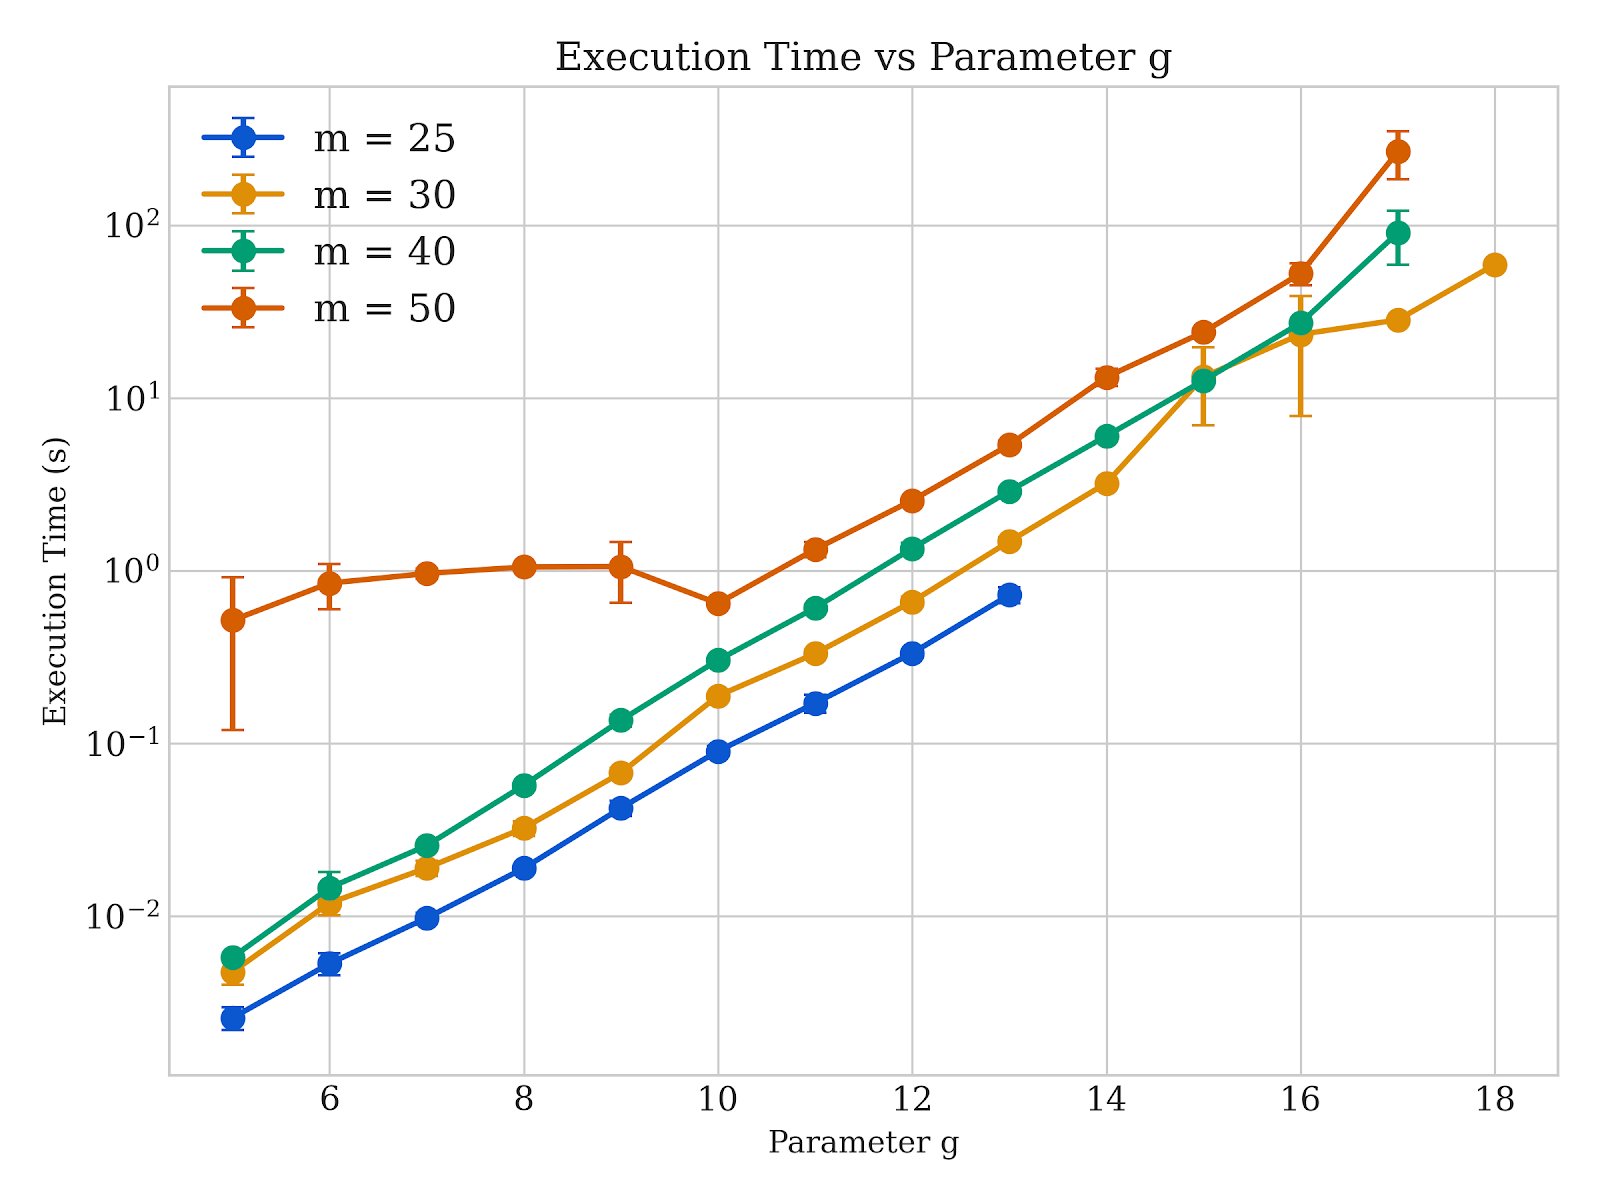
\includegraphics[width=0.72\textwidth]{FWHT1.1.png}
		\caption{Execution time as a function of circuit rank $g$ across different edge counts $m$ (log scale). The linear trajectories on the logarithmic axis reflect the $\bigO(2^g)$ dependence; all curves are parallel, and their vertical separation reflects the polynomial factor $m^{3}\log m$.}
		\label{fig:rq1_time}
	\end{figure}
	
	Figure~\ref{fig:rq1_time} confirms the $\bigO(2^g \cdot m^3 \log m)$ complexity predicted by Theorem~\ref{thm:time}: execution time grows exponentially with $g$ and the four curve families are visually parallel on the log scale. For $g\le 8$ all instances finish within one second; beyond $g=15$ runtimes reach tens to hundreds of seconds.
	
	The parallel trajectories arise from the separable factorization established in Proposition~\ref{prop:separable}. Taking logarithms of Eq.~\eqref{eq:complexity_factored} yields $\ln T(g,m) = (\ln 2) \cdot g + \varphi(m)$ where $\varphi(m) = 3\ln m + \ln\ln m + \ln C$. For a fixed~$m_0$, this is an affine function of $g$ with slope exactly $\ln 2 \approx 0.693$, independent of~$m_0$. The vertical separation between two curves at edge counts $m_1 > m_2$ is $\Delta\varphi = 3\ln(m_1/m_2) + \ln(\ln m_1 / \ln m_2)$, a quantity governed solely by the polynomial ratio of the edge counts, which accounts for the nearly uniform vertical gaps visible in the figure.
	
	\begin{figure}[H]
		\centering
		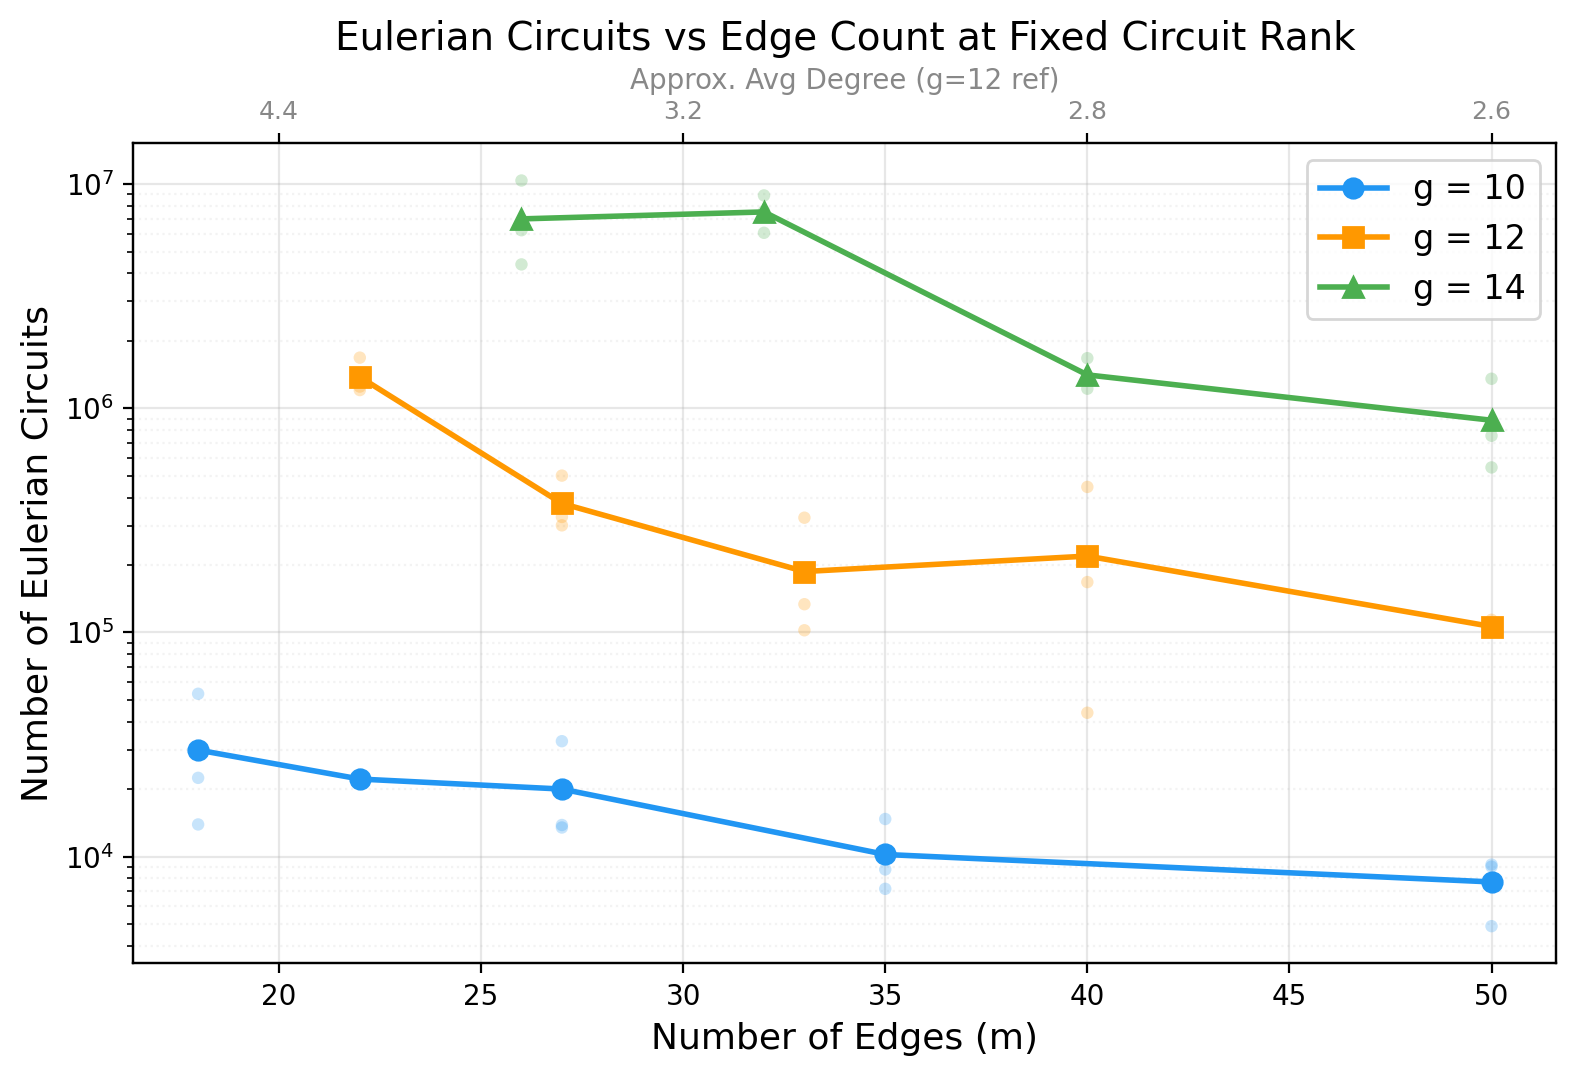
\includegraphics[width=0.72\textwidth]{FWHT1.2_new.png}
		\caption{Number of Eulerian circuits as a function of edge count $m$ at fixed circuit rank $g\in\{10,12,14\}$ (log scale). Each solid marker is the mean of three independent instances; translucent dots show individual values. The secondary $x$-axis reports approximate average degree $2m/n = 2m/(m-g+1)$ using $g=12$ as reference.}
		\label{fig:rq1_ec}
	\end{figure}
	
	Figure~\ref{fig:rq1_ec} isolates the influence of edge density on the Eulerian circuit count while holding topological complexity fixed. For every fixed $g$, the circuit count \emph{decreases} as $m$ grows: sparser graphs (larger $m$, lower average degree) admit fewer Eulerian circuits than denser graphs at the same~$g$. At $g=14$, for example, reducing the average degree from roughly $4.0$ ($m=26$) to $2.7$ ($m=50$) lowers the mean circuit count by more than one order of magnitude. Increasing $g$ by $2$ lifts the entire curve upward by roughly two orders of magnitude, consistent with the $2^g$ factor: fixing $m=50$, the mean count rises from $\approx 7\times10^{3}$ at $g=10$ to $\approx 10^{5}$ at $g=12$ and $\approx 10^{6}$ at $g=14$. The variance across instances is substantially larger at lower $m$, where the graphs are denser and structurally more diverse; the coefficient of variation narrows as $m$ increases and graphs become more tree-like.
	
	These results show that circuit rank $g$ is the dominant driver of combinatorial explosion, while edge density modulates the count within the regime set by~$g$. This separation mirrors the factorization in Eq.~\eqref{eq:complexity_factored} and further validates the FPT character of the algorithm.
	
	\subsection{RQ2: Comparison with Backtracking}
	\label{subsec:crossover}
	
	To evaluate when the FWHT-based algebraic method becomes competitive against classical backtracking enumeration, we designed a controlled experiment spanning four graph families with varying density and structure.
	
	\subsubsection{Experimental Setup}
	
	We generated Eulerian graphs across four families using a \emph{sliding-$N$} strategy, where the number of nodes~$N$ is chosen per family to keep the DFS baseline tractable at lower circuit rank values while allowing the scaling divergence to emerge at higher values.
	
	\begin{enumerate}
		\item \textbf{Sparse (Havel--Hakimi style, $N = 15$--$30$):} Starting from a Hamiltonian cycle, we incrementally add long random cycles (length 5--8) to reach the target circuit rank. This produces graphs with high $N$, low edge density, and limited branching.
		\item \textbf{Medium (Tangled Web, $N = 8$--$10$):} A base cycle is overlaid with short random cycles (triangles and squares), yielding moderate density and overlapping cycle structure.
		\item \textbf{Dense (Extreme Overlap, $N = 6$--$7$):} A base cycle is flooded with triangles on a minimal node set, maximizing edge overlap and DFS branching factor.
		\item \textbf{Tangled ($N = 7$, $g = 10$--$21$):} An extension of the dense family pushed to higher circuit rank ($g$ up to~$21$), designed to stress-test both methods at the performance frontier.
	\end{enumerate}
	
	All graphs satisfy the Eulerian condition (all degrees even, single connected component). The DFS baseline uses exhaustive backtracking with a 600-second timeout; when the timeout is reached, partial progress is recorded and the total DFS runtime is extrapolated using the rate of closed trails discovered per second and the known circuit count from FWHT. The FWHT method uses the parallel OpenMP implementation described in Section~\ref{subsec:thread_local}. Across the four families, we tested 27 graph instances with circuit rank $g$ ranging from 6 to 21 and edge counts $m$ from 13 to~45.
	
	\textbf{Caveat on the DFS baseline.} Our backtracking implementation is a straightforward recursive enumerator without advanced pruning heuristics such as bridge detection, Fleury-type edge ordering, or memoization of partial states. A more sophisticated backtracking solver could shift the crossover point to higher values of~$g$. However, because the DFS runtime is fundamentally coupled to the \emph{output size} (which grows super-exponentially with $g$), any pruning strategy can only reduce the constant factor, not the asymptotic growth rate. The crossover trends observed below---particularly the exponential divergence beyond the crossover---are therefore expected to hold qualitatively for optimized backtracking implementations as well, albeit at shifted threshold values.
	
	\subsubsection{Results}
	
	\paragraph{Runtime vs.\ Circuit Rank.}
	Figure~\ref{fig:rq2_genus} plots computation time (log scale) against circuit rank for both methods across all four families. The FWHT curves (solid lines) exhibit the expected $\bigO(2^g \cdot \text{poly}(m))$ scaling: they rise steadily and predictably, with all four families producing closely grouped curves at the same circuit rank value---confirming that FWHT runtime is governed primarily by $g$ rather than graph structure. In contrast, the DFS curves (dashed lines) are highly sensitive to graph density. Sparse graphs remain tractable for DFS across the tested range ($g \le 16$), while medium-density graphs begin timing out around $g = 14$--$15$, and the Tangled family exceeds the 600\,s limit at $g = 18$, with extrapolated runtimes reaching $10^7$\,s at $g = 21$.
	
	\begin{figure}[H]
		\centering
		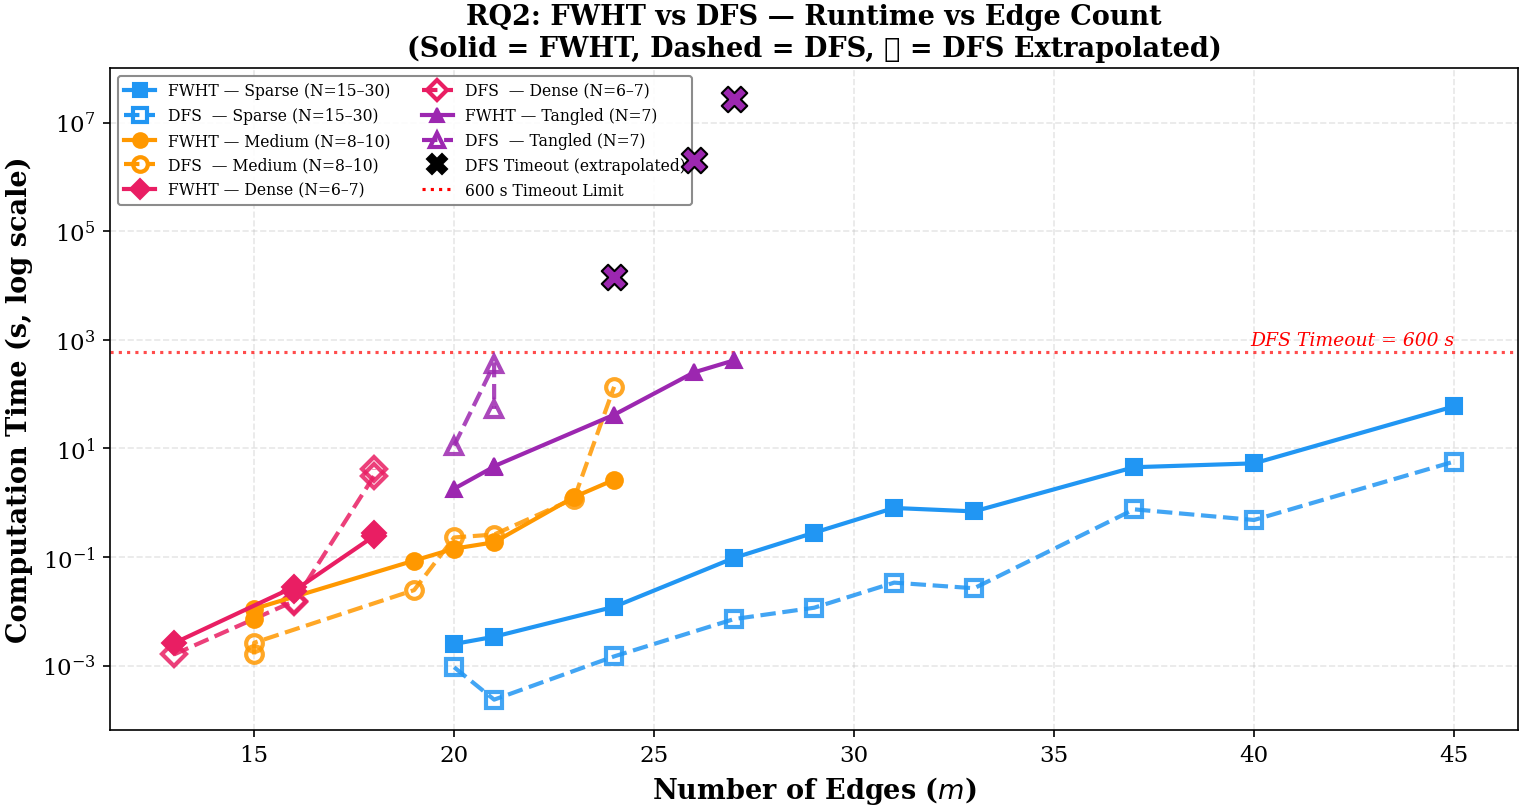
\includegraphics[width=0.82\textwidth]{RQ2_3.png}
		\caption{Computation time (log scale) vs.\ circuit rank for FWHT (solid) and DFS (dashed) across four graph families. {\large$\times$} markers denote DFS instances that exceeded the 600\,s timeout, with runtime extrapolated from partial progress. The FWHT curves cluster together regardless of density, while DFS diverges sharply across families.}
		\label{fig:rq2_genus}
	\end{figure}
	
	\paragraph{Runtime vs.\ Edge Count.}
	Figure~\ref{fig:rq2_edges} re-plots the same data against the number of edges~$m$, revealing how the two methods respond to raw problem size. The FWHT method shows a smooth, family-independent scaling trend: doubling the edge count increases runtime by a predictable polynomial factor. DFS, however, displays an erratic, family-dependent response---at $m = 24$--$27$ edges, the Tangled family's DFS runtime jumps from ${\sim}50$\,s to an extrapolated $10^7$\,s, while the Sparse family at the same or higher $m$ values completes in under~6\,s.
	
	\begin{figure}[H]
		\centering
		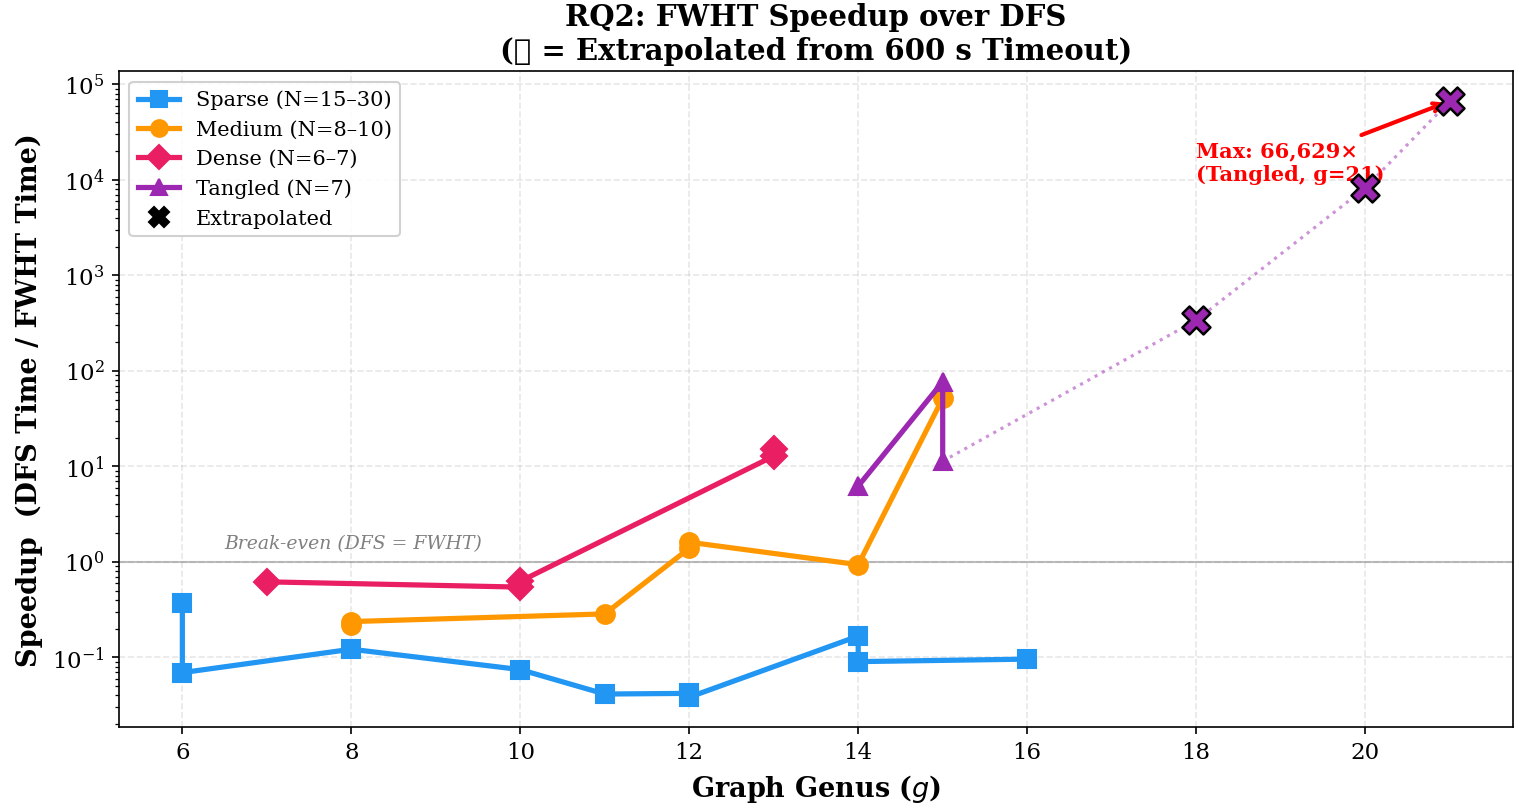
\includegraphics[width=0.82\textwidth]{RQ2_2.png}
		\caption{Computation time (log scale) vs.\ number of edges for FWHT (solid) and DFS (dashed). At moderate edge counts ($m \approx 20$--$27$), DFS runtimes diverge by up to six orders of magnitude depending on graph density, while FWHT remains predictable.}
		\label{fig:rq2_edges}
	\end{figure}
	
	\paragraph{Speedup Analysis.}
	Figure~\ref{fig:rq2_speedup} shows the ratio of DFS time to FWHT time as a function of circuit rank. Three distinct regimes emerge. In the \emph{DFS-favorable regime} ($g \le 8$--$10$), DFS is 3--10$\times$ faster than FWHT for sparse graphs due to its negligible constant overhead. In the \emph{crossover regime} ($g \approx 10$--$14$), the speedup crosses the break-even line for medium and dense families; the exact crossover depends on density ($g \approx 12$ for medium, $g \approx 10$ for dense). In the \emph{FWHT-dominant regime} ($g \ge 14$), the speedup grows exponentially, reaching approximately $66{,}629\times$ for the Tangled family at $g = 21$ (extrapolated), where FWHT completes in 420\,s while DFS would require an estimated 324 days.
	
	This exponential divergence has a clear algorithmic explanation: DFS enumerates individual Eulerian circuits, whose count grows super-exponentially with~$g$, while the FWHT-based method performs exactly $2^g$ matrix power computations regardless of how many circuits exist. The DFS runtime is thus coupled to the \emph{output size} (number of circuits), whereas the FWHT runtime depends only on the \emph{parameter size} ($g$ and $m$).
	
	\begin{figure}[H]
		\centering
		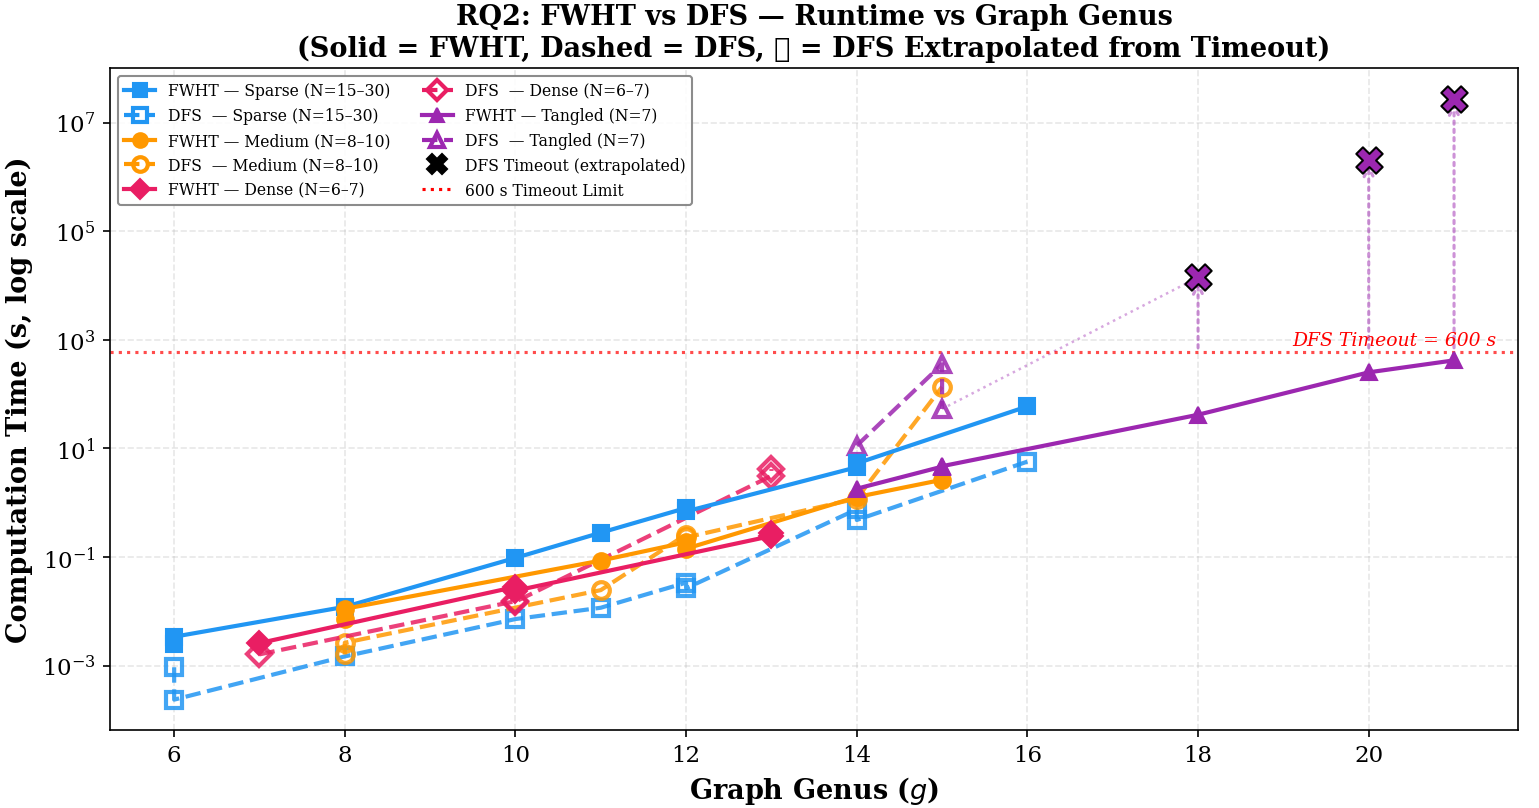
\includegraphics[width=0.82\textwidth]{RQ2_1.png}
		\caption{Speedup of FWHT over DFS (log scale) vs.\ circuit rank. The gray line marks break-even ($1\times$). {\large$\times$} markers indicate extrapolated values from DFS timeouts. The maximum speedup reaches ${\approx}66{,}629\times$ for the Tangled family at $g = 21$.}
		\label{fig:rq2_speedup}
	\end{figure}
	
	\paragraph{Complete Data.}
	Table~\ref{tab:rq2_data} presents the full experimental data across all 27 instances. Of these, 24 completed within the DFS timeout and 3 required extrapolation (all from the Tangled family at $g = 18, 20, 21$). The extrapolated DFS runtimes for these three instances are approximately 3.9~hours, 24~days, and 324~days, respectively, while FWHT completes them in 42\,s, 253\,s, and 420\,s.
	
	% Define row colors for the table
	\definecolor{timeoutred}{RGB}{255,204,204}
	\definecolor{speedupgreen}{RGB}{204,255,204}
	\definecolor{speedupyellow}{RGB}{255,255,204}
	
	\begin{table}[H]
		\centering
		\caption{Complete experimental data for all 27 graph instances. Shaded rows indicate: {\colorbox{timeoutred}{red}} = DFS timeout with extrapolated runtime; {\colorbox{speedupgreen}{green}} = speedup exceeding $100\times$; {\colorbox{speedupyellow}{yellow}} = speedup exceeding~$10\times$.}
		\label{tab:rq2_data}
		\resizebox{\textwidth}{!}{%
			\begin{tabular}{@{}llrrrrrrr@{}}
				\toprule
				\textbf{Family} & \textbf{File} & $\boldsymbol{N}$ & $\boldsymbol{M}$ & $\boldsymbol{g}$ & \textbf{FWHT (s)} & \textbf{DFS (s)} & \textbf{Status} & \textbf{Speedup} \\
				\midrule
				Sparse & sparse\_n15\_g5  & 15 & 20 &  6 & 0.0025 & 0.0009  & OK & $0.4\times$ \\
				Sparse & sparse\_n16\_g6  & 16 & 21 &  6 & 0.0034 & 0.0002  & OK & $0.1\times$ \\
				Sparse & sparse\_n17\_g7  & 17 & 24 &  8 & 0.0121 & 0.0015  & OK & $0.1\times$ \\
				Sparse & sparse\_n18\_g8  & 18 & 27 &  8 & 0.0964 & 0.0072  & OK & $0.1\times$ \\
				Sparse & sparse\_n19\_g9  & 19 & 29 & 11 & 0.2809 & 0.0116  & OK & $0.0\times$ \\
				Sparse & sparse\_n20\_g10 & 20 & 31 & 12 & 0.8010 & 0.0337  & OK & $0.0\times$ \\
				Sparse & sparse\_n22\_g11 & 22 & 33 & 12 & 0.6924 & 0.0266  & OK & $0.0\times$ \\
				Sparse & sparse\_n24\_g12 & 24 & 37 & 14 & 4.51   & 0.7558  & OK & $0.2\times$ \\
				Sparse & sparse\_n27\_g13 & 27 & 40 & 14 & 5.32   & 0.4812  & OK & $0.1\times$ \\
				Sparse & sparse\_n30\_g14 & 30 & 45 & 16 & 59.60  & 5.73    & OK & $0.1\times$ \\
				\midrule
				Medium & medium\_n8\_g6   &  8 & 15 &  8 & 0.0073 & 0.0016  & OK & $0.2\times$ \\
				Medium & medium\_n8\_g7   &  8 & 15 &  8 & 0.0111 & 0.0026  & OK & $0.2\times$ \\
				Medium & medium\_n9\_g8   &  9 & 19 & 11 & 0.0860 & 0.0246  & OK & $0.3\times$ \\
				Medium & medium\_n10\_g10 & 10 & 21 & 12 & 0.1870 & 0.2598  & OK & $1.4\times$ \\
				Medium & medium\_n9\_g9   &  9 & 20 & 12 & 0.1425 & 0.2294  & OK & $1.6\times$ \\
				Medium & medium\_n10\_g11 & 10 & 23 & 14 & 1.27   & 1.19    & OK & $0.9\times$ \\
				\rowcolor{speedupyellow}
				Medium & medium\_n10\_g12 & 10 & 24 & 15 & 2.65   & 136.66  & OK & $51.6\times$ \\
				\midrule
				Dense  & dense\_n7\_g6    &  7 & 13 &  7 & 0.0026 & 0.0016  & OK & $0.6\times$ \\
				Dense  & dense\_n7\_g7    &  7 & 16 & 10 & 0.0282 & 0.0154  & OK & $0.5\times$ \\
				Dense  & dense\_n7\_g8    &  7 & 16 & 10 & 0.0240 & 0.0151  & OK & $0.6\times$ \\
				\rowcolor{speedupyellow}
				Dense  & dense\_n6\_g10   &  6 & 18 & 13 & 0.2439 & 3.13    & OK & $12.8\times$ \\
				\rowcolor{speedupyellow}
				Dense  & dense\_n6\_g9    &  6 & 18 & 13 & 0.2740 & 4.16    & OK & $15.2\times$ \\
				\midrule
				Tangled & tangled\_n7\_g10 &  7 & 20 & 14 & 1.81   & 11.29   & OK & $6.2\times$ \\
				\rowcolor{speedupyellow}
				Tangled & tangled\_n7\_g11 &  7 & 21 & 15 & 4.62   & 356.02  & OK & $77.0\times$ \\
				\rowcolor{speedupyellow}
				Tangled & tangled\_n7\_g12 &  7 & 21 & 15 & 4.71   & 53.43   & OK & $11.3\times$ \\
				\rowcolor{timeoutred}
				Tangled & tangled\_n7\_g13 &  7 & 24 & 18 & 41.77  & $\approx$3.9\,h   & TIMEOUT & $\approx$$339\times$ \\
				\rowcolor{timeoutred}
				Tangled & tangled\_n7\_g14 &  7 & 26 & 20 & 252.50 & $\approx$24.0\,days & TIMEOUT & $\approx$$8{,}199\times$ \\
				\rowcolor{timeoutred}
				Tangled & tangled\_n7\_g15 &  7 & 27 & 21 & 419.90 & $\approx$323.8\,days & TIMEOUT & $\approx$$66{,}629\times$ \\
				\bottomrule
			\end{tabular}%
		}
	\end{table}
	
	\subsubsection{Analysis}
	
	These results refine the crossover picture in three important ways.
	
	First, \textbf{the crossover is density-dependent, not universal}. The multi-family design reveals that the crossover circuit rank varies significantly: sparse graphs with high $N$ and low branching factor remain DFS-favorable throughout the tested range ($g \le 16$), while dense graphs with maximal edge overlap cross over as early as $g = 10$. This is expected: DFS runtime depends not only on the number of Eulerian circuits (which grows combinatorially with $g$) but also on the per-node branching factor, which is amplified by density. The practical implication is that users should consider both circuit rank and edge density when choosing between the two methods.
	
	Second, \textbf{FWHT scaling is structure-agnostic}. Across all four families, the FWHT runtime at a given circuit rank varies by less than one order of magnitude, and this variation is attributable to differences in edge count~$m$ (which affects the matrix dimension $2m$) rather than graph topology. This confirms the FPT nature of the algorithm: its runtime is controlled by the parameter $g$ via the $2^g$ factor, with only polynomial dependence on the input size, as predicted by Theorem~\ref{thm:time}.
	
	Third, \textbf{the speedup grows exponentially beyond the crossover}. Once the crossover is passed, each additional unit of circuit rank roughly doubles the speedup factor. This exponential divergence arises because DFS enumerates individual circuits (whose count grows super-exponentially with $g$), while FWHT performs a fixed number of $2^g$ matrix power computations regardless of how many circuits exist. We reiterate that the specific crossover values reported here ($g \approx 10$--$12$ for dense graphs) are measured against an unoptimized backtracking baseline; an optimized DFS implementation with pruning heuristics would likely shift these thresholds upward by several units without altering the qualitative picture.
	
	\subsection{RQ3: Effect of Graph Size at Fixed Circuit Rank}
	\label{subsec:exp3}
	
	The complexity analysis in Section~\ref{sec:complexity} predicts that, at a fixed circuit rank~$g$, the runtime scales as $\bigO(m^3 \log m)$ in the number of edges. RQ3 isolates this polynomial factor by holding $g$ constant and varying the edge count~$m$ across three structurally distinct graph families:
	
	\begin{enumerate}
		\item \textbf{Cactus graphs:} $g$ cycles sharing only cut-vertices. Each cycle is attached to a randomly chosen existing vertex, producing a tree-like global structure with locally disjoint cycles.
		\item \textbf{Chain-of-cycles:} $g$ cycles linked sequentially, where the last vertex of one cycle is identified with the first vertex of the next. This yields a linear, path-like backbone.
		\item \textbf{Random Eulerian graphs:} Starting from a spanning path, $g$ random back-edges are inserted to achieve the target circuit rank, and parity-violating vertices are repaired by adding parallel edges. This produces irregular, less structured topologies.
	\end{enumerate}
	
	For each combination of family, circuit rank $g \in \{8, 10, 12\}$, and target edge count~$m$, we generated 3 independent instances and report mean values with error bars indicating the range across repetitions. A per-instance timeout of 600\,s was imposed.
	
	\subsubsection{Runtime Scaling}
	
	Figure~\ref{fig:rq3_time} plots execution time against edge count for each family at the three circuit rank values. At each fixed~$g$, the data points for all three families closely track the fitted curve $C \cdot m^3 \log m$ (dashed line), confirming the predicted polynomial dependence. For $g = 8$, all instances with $m \le 250$ complete within 35\,s. For $g = 10$, runtimes reach approximately 300\,s at $m = 300$. At $g = 12$, several instances with $m \ge 260$ approach or exceed the 600\,s timeout, consistent with the larger constant factor $2^{12} = 4096$ multiplying the polynomial term.
	
	Across all three panels, the three families produce nearly overlapping runtime curves at the same~$g$, reinforcing the conclusion from RQ2 that the FWHT-based algorithm is structure-agnostic: its runtime is governed by the parameters $(g, m)$ and is insensitive to the internal cycle topology of the graph.
	
	\begin{figure}[H]
		\centering
		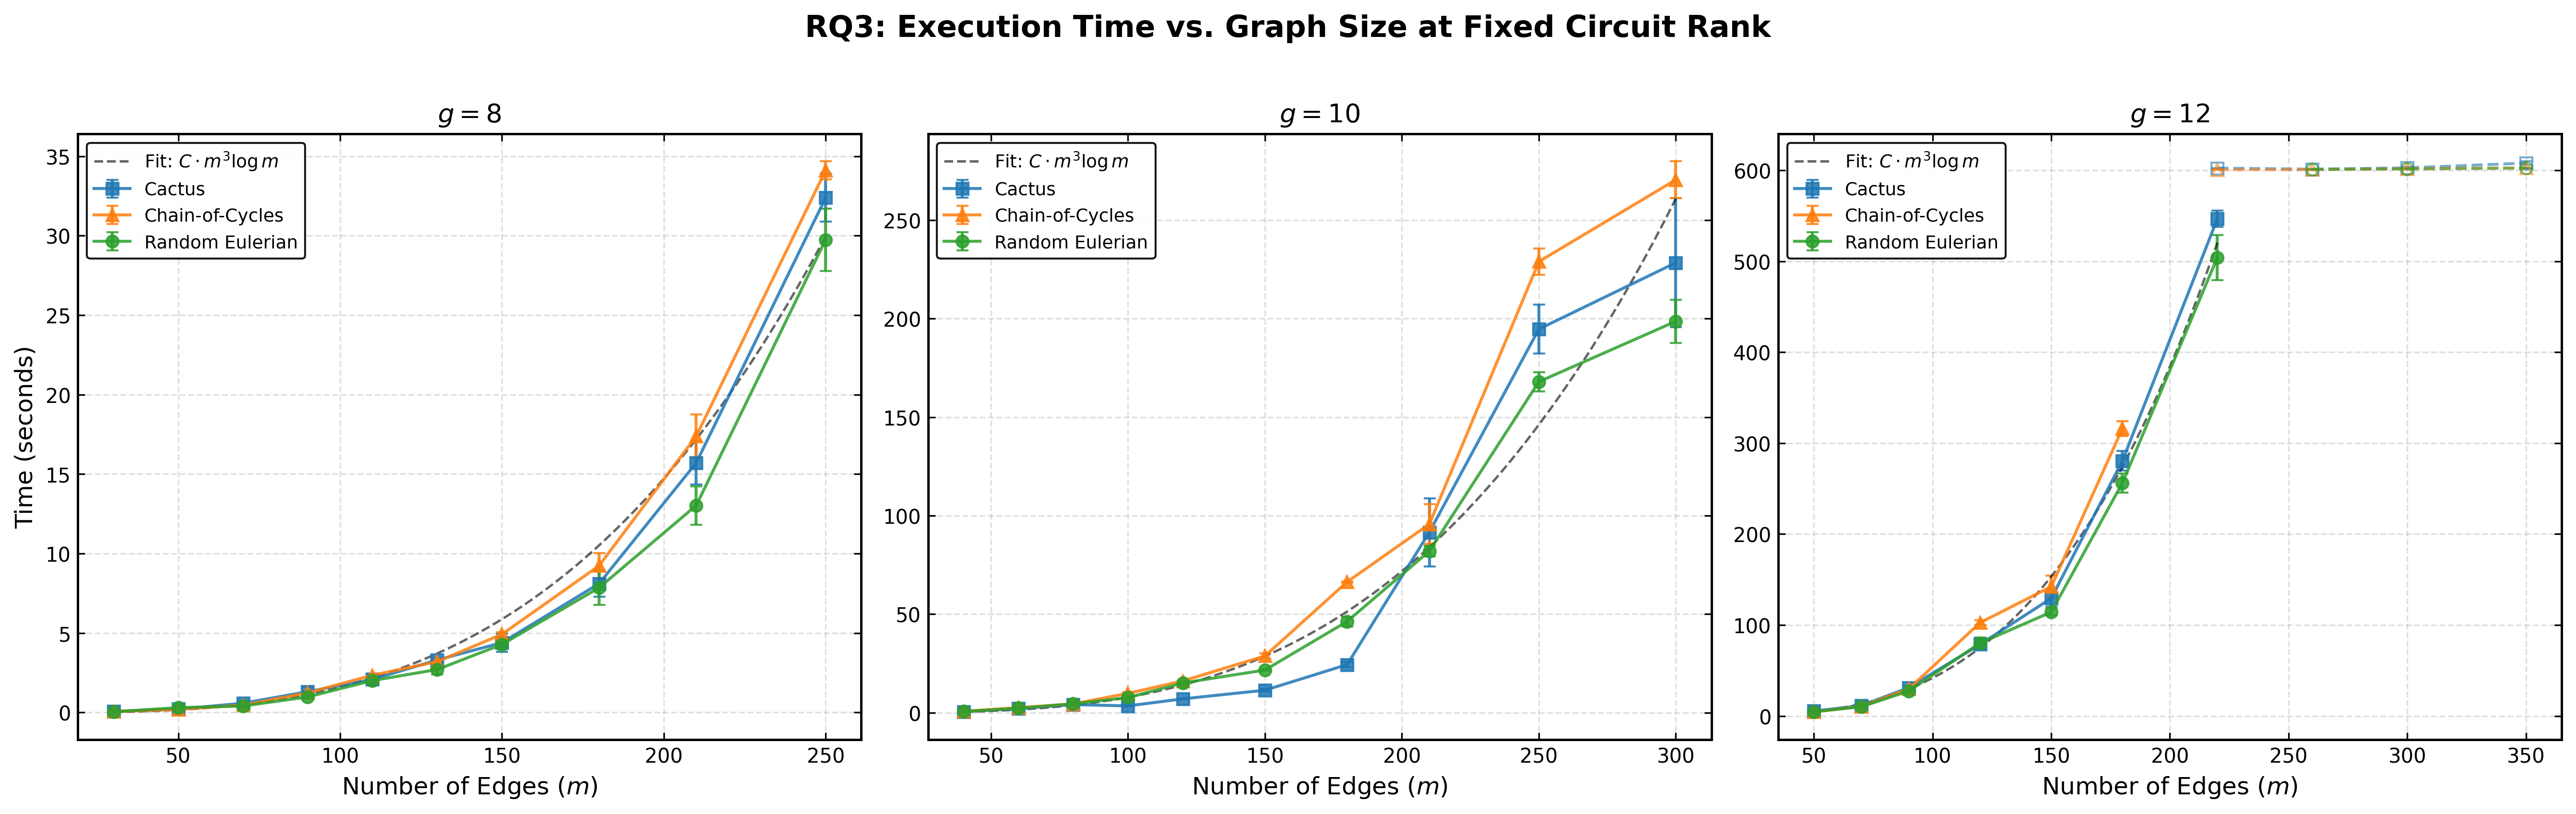
\includegraphics[width=\textwidth]{RQ3_time_vs_M.png}
		\caption{Execution time vs.\ number of edges~$m$ at fixed circuit rank $g \in \{8, 10, 12\}$ for three graph families. The dashed curve shows the least-squares fit to $C \cdot m^3 \log m$. Error bars span the range of 3 independent instances. Flat segments at the top of the $g = 12$ panel indicate instances that reached the 600\,s timeout.}
		\label{fig:rq3_time}
	\end{figure}
	
	\subsubsection{Complexity Validation via Normalized Time}
	
	To validate the $m^3 \log m$ scaling law more rigorously, Figure~\ref{fig:rq3_normalized} plots the \emph{normalized time} $T / (m^3 \log m)$ against the edge count. If the theoretical complexity accurately describes the runtime, this ratio should remain approximately constant across all values of~$m$ for a given~$g$.
	
	For $g = 8$, the normalized time is virtually flat across the entire range $m \in [30, 250]$, with all three families converging to a common constant near $3 \times 10^{-4}$, providing strong empirical validation of the $m^3 \log m$ model. For $g = 10$, the normalized ratio remains stable in the range $[1.0, 1.8] \times 10^{-3}$, with mild fluctuations attributable to cache effects and thread scheduling variance. The roughly $4\times$ increase in the constant from $g = 8$ to $g = 10$ is consistent with the factor $2^{10}/2^8 = 4$ predicted by the $2^g$ term. For $g = 12$, the normalized values cluster around $[5, 8] \times 10^{-3}$ for $m \le 220$, again reflecting the expected $4\times$ jump. At larger $m$, the chain-of-cycles family exhibits elevated normalized times, likely caused by reduced sparsity in the twisted matrices at high edge counts, which diminishes the effectiveness of the zero-entry bypass in the matrix multiplication kernel.
	
	\begin{figure}[H]
		\centering
		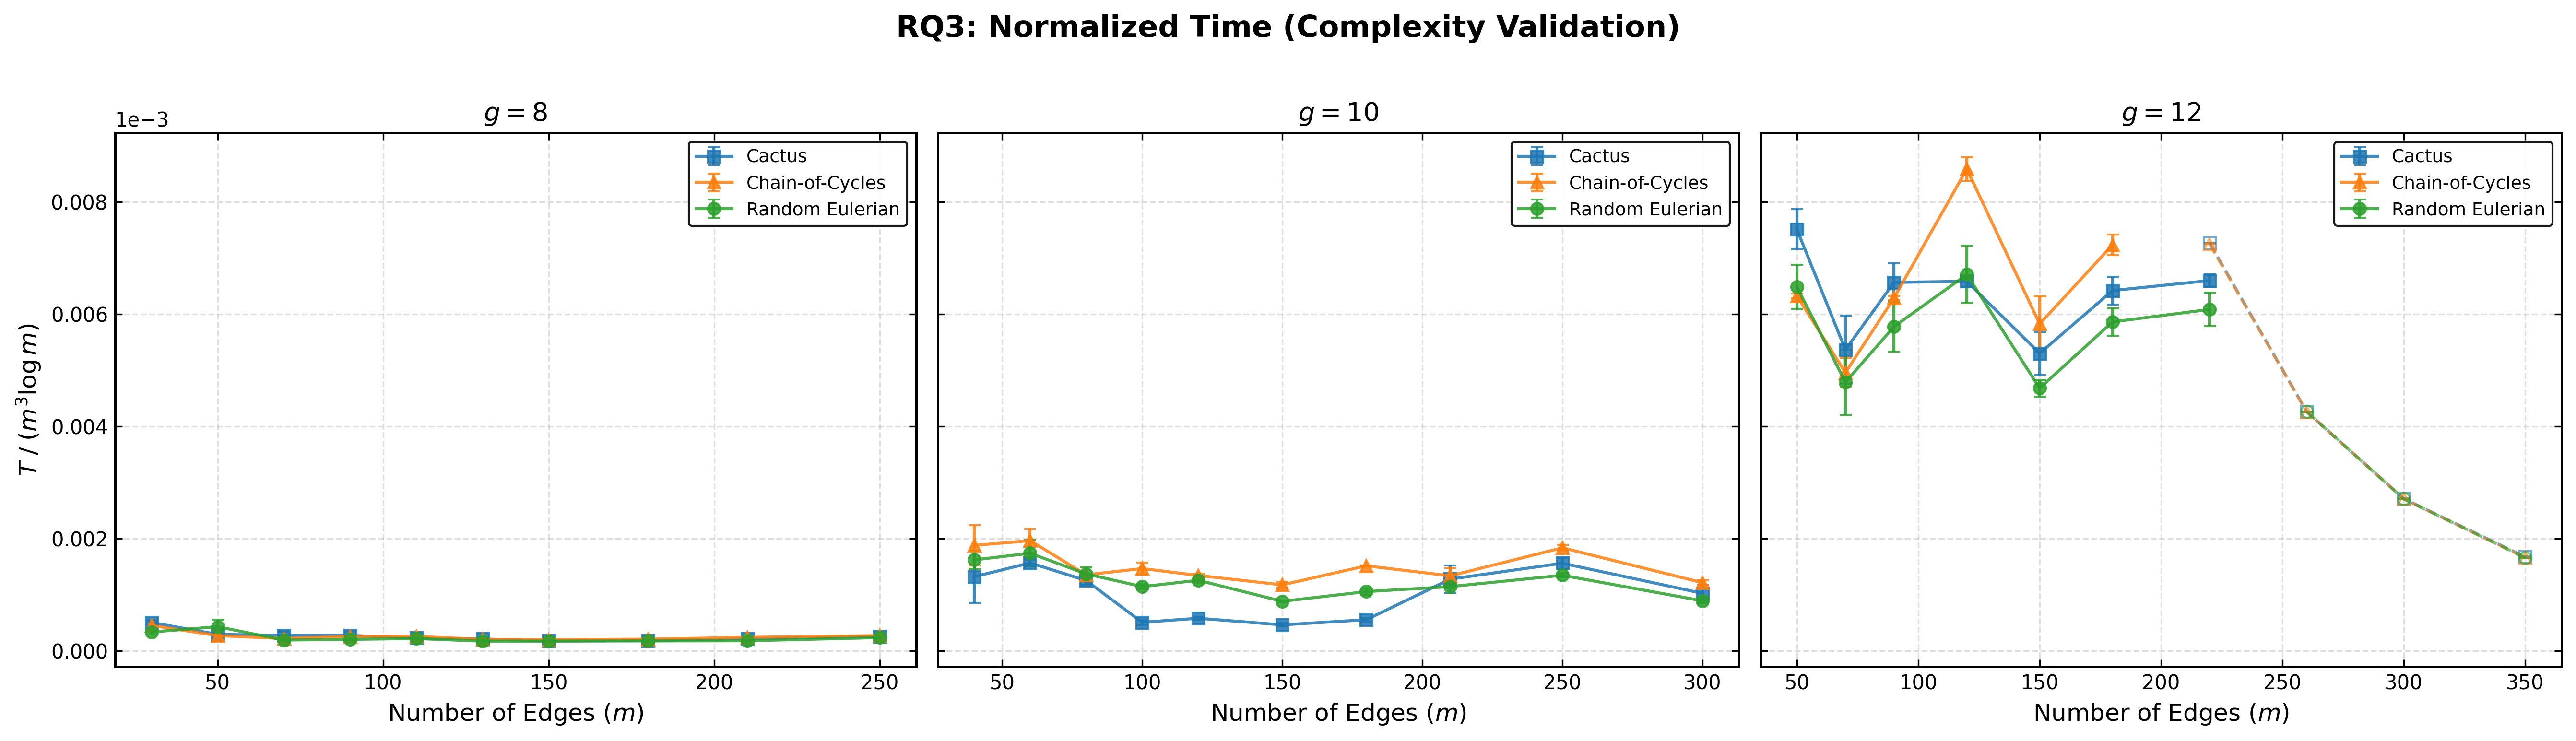
\includegraphics[width=\textwidth]{RQ3_normalized.png}
		\caption{Normalized time $T / (m^3 \log m)$ vs.\ number of edges. A constant trend validates the $\bigO(m^3 \log m)$ complexity model. The vertical scale increases by approximately $4\times$ from each panel to the next, matching the $2^g$ factor. Dashed markers at $g = 12$ correspond to instances that timed out.}
		\label{fig:rq3_normalized}
	\end{figure}
	
	\subsubsection{Eulerian Circuit Count vs.\ Graph Size}
	
	Figure~\ref{fig:rq3_ec} shows the number of Eulerian circuits (log scale) as a function of edge count for the three families. Unlike the runtime, which is structure-agnostic, the circuit count depends strongly on graph topology.
	
	\textbf{Chain-of-cycles} graphs exhibit a nearly constant circuit count independent of~$m$ at each fixed~$g$: the count equals $2^g$ when all cycles have odd length, and varies by small factors otherwise. This behavior reflects the sequential topology, where each cycle contributes an independent binary choice of traversal direction, and these choices are decoupled by the chain structure.
	
	\textbf{Cactus} graphs show a decreasing trend in circuit count as $m$ increases. At small~$m$, the cycles are short, producing high edge overlap and many distinct traversal orders. As $m$ grows with $g$ held fixed, the additional edges are distributed among the $g$ cycles, lengthening them and reducing the combinatorial freedom at each vertex.
	
	\textbf{Random Eulerian} graphs display intermediate counts with higher variance, reflecting the structural diversity of the random generation process.
	
	This separation between computational cost (governed by $g$ and~$m$) and combinatorial output (governed by topology) further validates the FPT character of the algorithm: the hardness parameter is the circuit rank, not the structure or size of the graph.
	
	\begin{figure}[H]
		\centering
		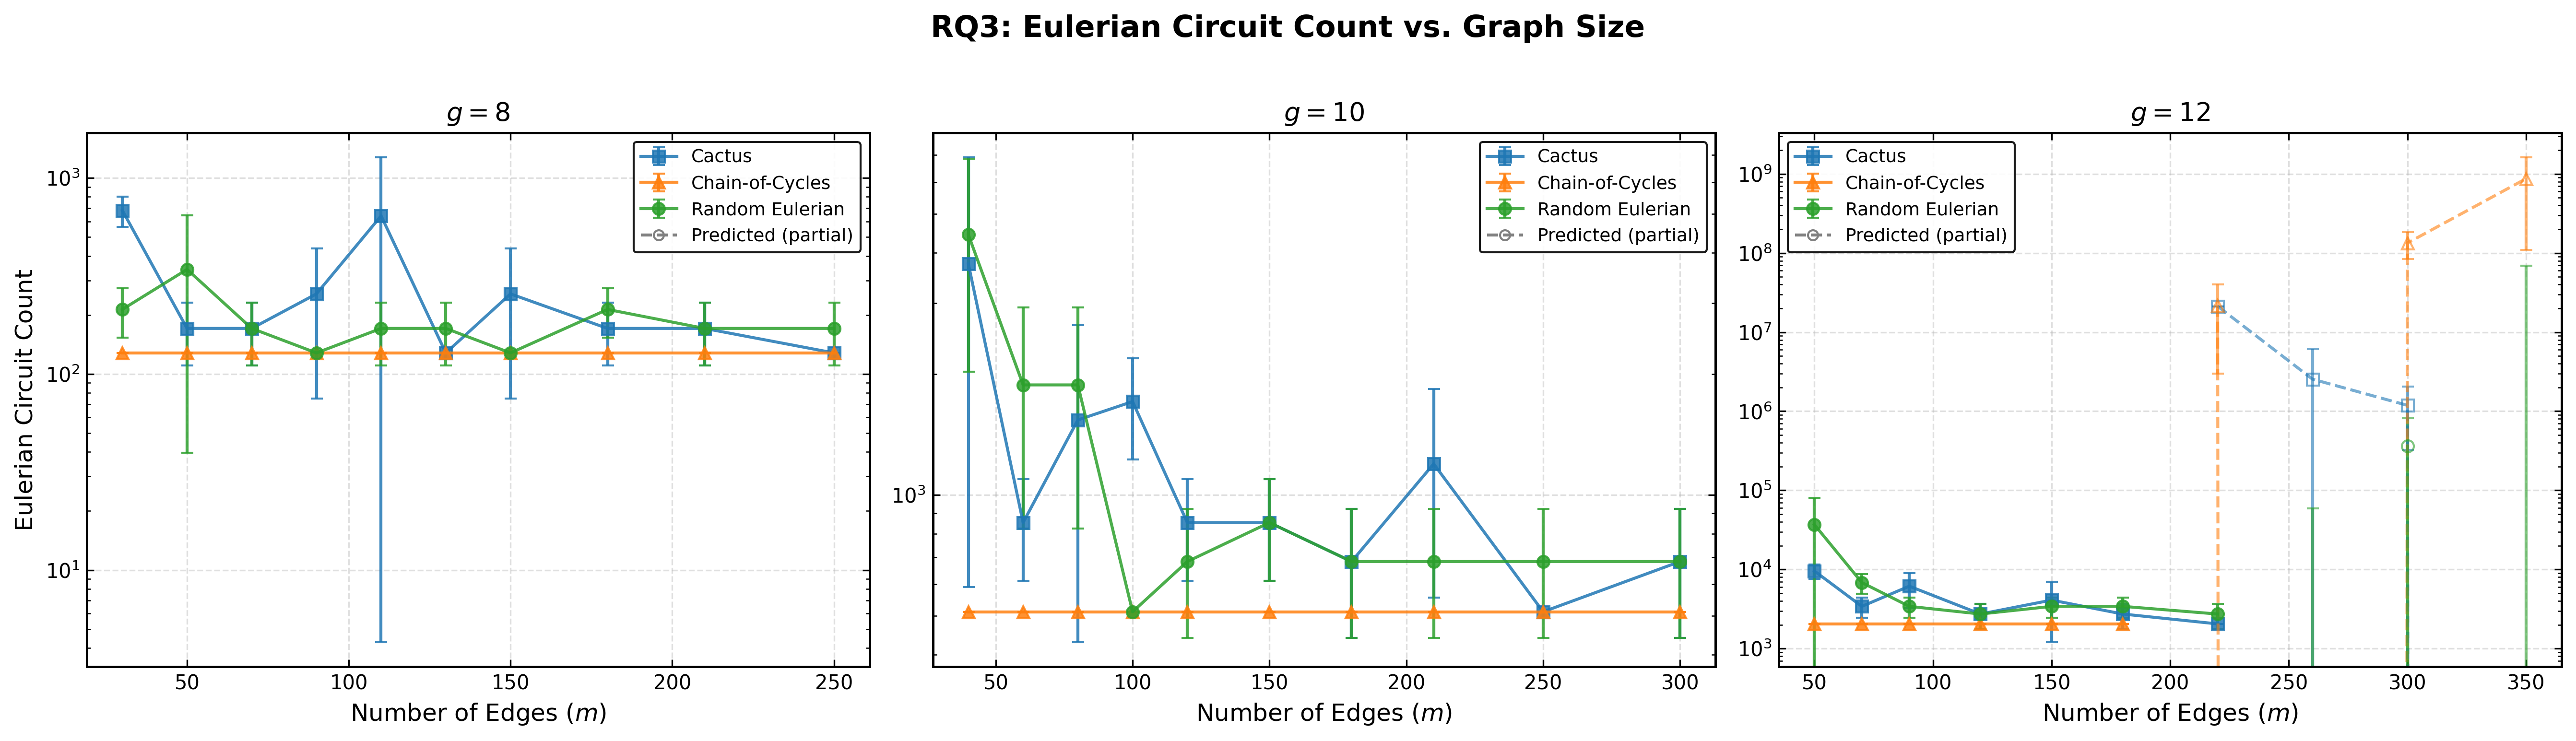
\includegraphics[width=\textwidth]{RQ3_ec_count.png}
		\caption{Eulerian circuit count (log scale) vs.\ number of edges at fixed circuit rank $g \in \{8, 10, 12\}$. Chain-of-cycles graphs (orange) maintain a nearly constant count; cactus graphs (blue) show a decreasing trend; random Eulerian graphs (green) exhibit intermediate values with higher variance. Dashed markers at $g = 12$ indicate partial results from timed-out instances.}
		\label{fig:rq3_ec}
	\end{figure}
	
	\subsection{RQ4: Parallel Scaling}
	\label{sec:rq4}
	
	The $2^g$ state evaluations in Algorithm~\ref{alg:eulerian_fwht} are independent and therefore amenable to data-parallel execution. RQ4 investigates how effectively the OpenMP parallelization (Section~\ref{subsec:thread_local}) exploits this independence by measuring speedup, parallel efficiency, and the serial bottleneck fraction across multiple problem sizes.
	
	\subsubsection{Experimental Setup}
	
	We generated four cactus-graph benchmarks with increasing circuit rank and edge count: $(g, m) \in \{(10, 40),\; (12, 45),\; (13, 50),\; (14, 55)\}$, corresponding to $2^{10} = 1024$ through $2^{14} = 16384$ independent state evaluations. For each $(g, m)$ pair, we ran the solver at thread counts $p \in \{1, 2, 4, 8, 16, 32\}$ with 3 repetitions per configuration, recording mean wall-clock time. All experiments were conducted on a single multi-core machine with shared-memory access.
	
	\subsubsection{Speedup}
	
	Figure~\ref{fig:rq4_speedup_new} presents the speedup ratio $S(p) = T_1 / T_p$ as a function of thread count for each problem size. The scaling behavior varies markedly with problem size. The smallest instance ($g = 10$, $T_1 = 3.67$\,s) achieves a peak speedup of $10.3\times$ at 16 threads before degrading to $9.5\times$ at 32 threads, a consequence of the sub-second per-thread workload being dominated by scheduling overhead. The $g = 12$ instance ($T_1 = 50.4$\,s) reaches $24.9\times$ at 32 threads, exhibiting superlinear behavior discussed further below. The two larger instances ($g = 13$ and $g = 14$) exhibit progressively more conservative scaling: $16.6\times$ and $11.1\times$ at 32 threads, respectively.
	
	Notably, the $g = 14$ instance has the largest absolute workload ($T_1 = 404.4$\,s) yet the lowest relative speedup. This inversion is attributable to the larger per-state matrix dimension ($2m = 110$): the $110 \times 110$ matrix exponentiation creates a working set that exceeds per-core L2 cache capacity when distributed across many threads, increasing memory bandwidth contention.
	
	\begin{figure}[H]
		\centering
		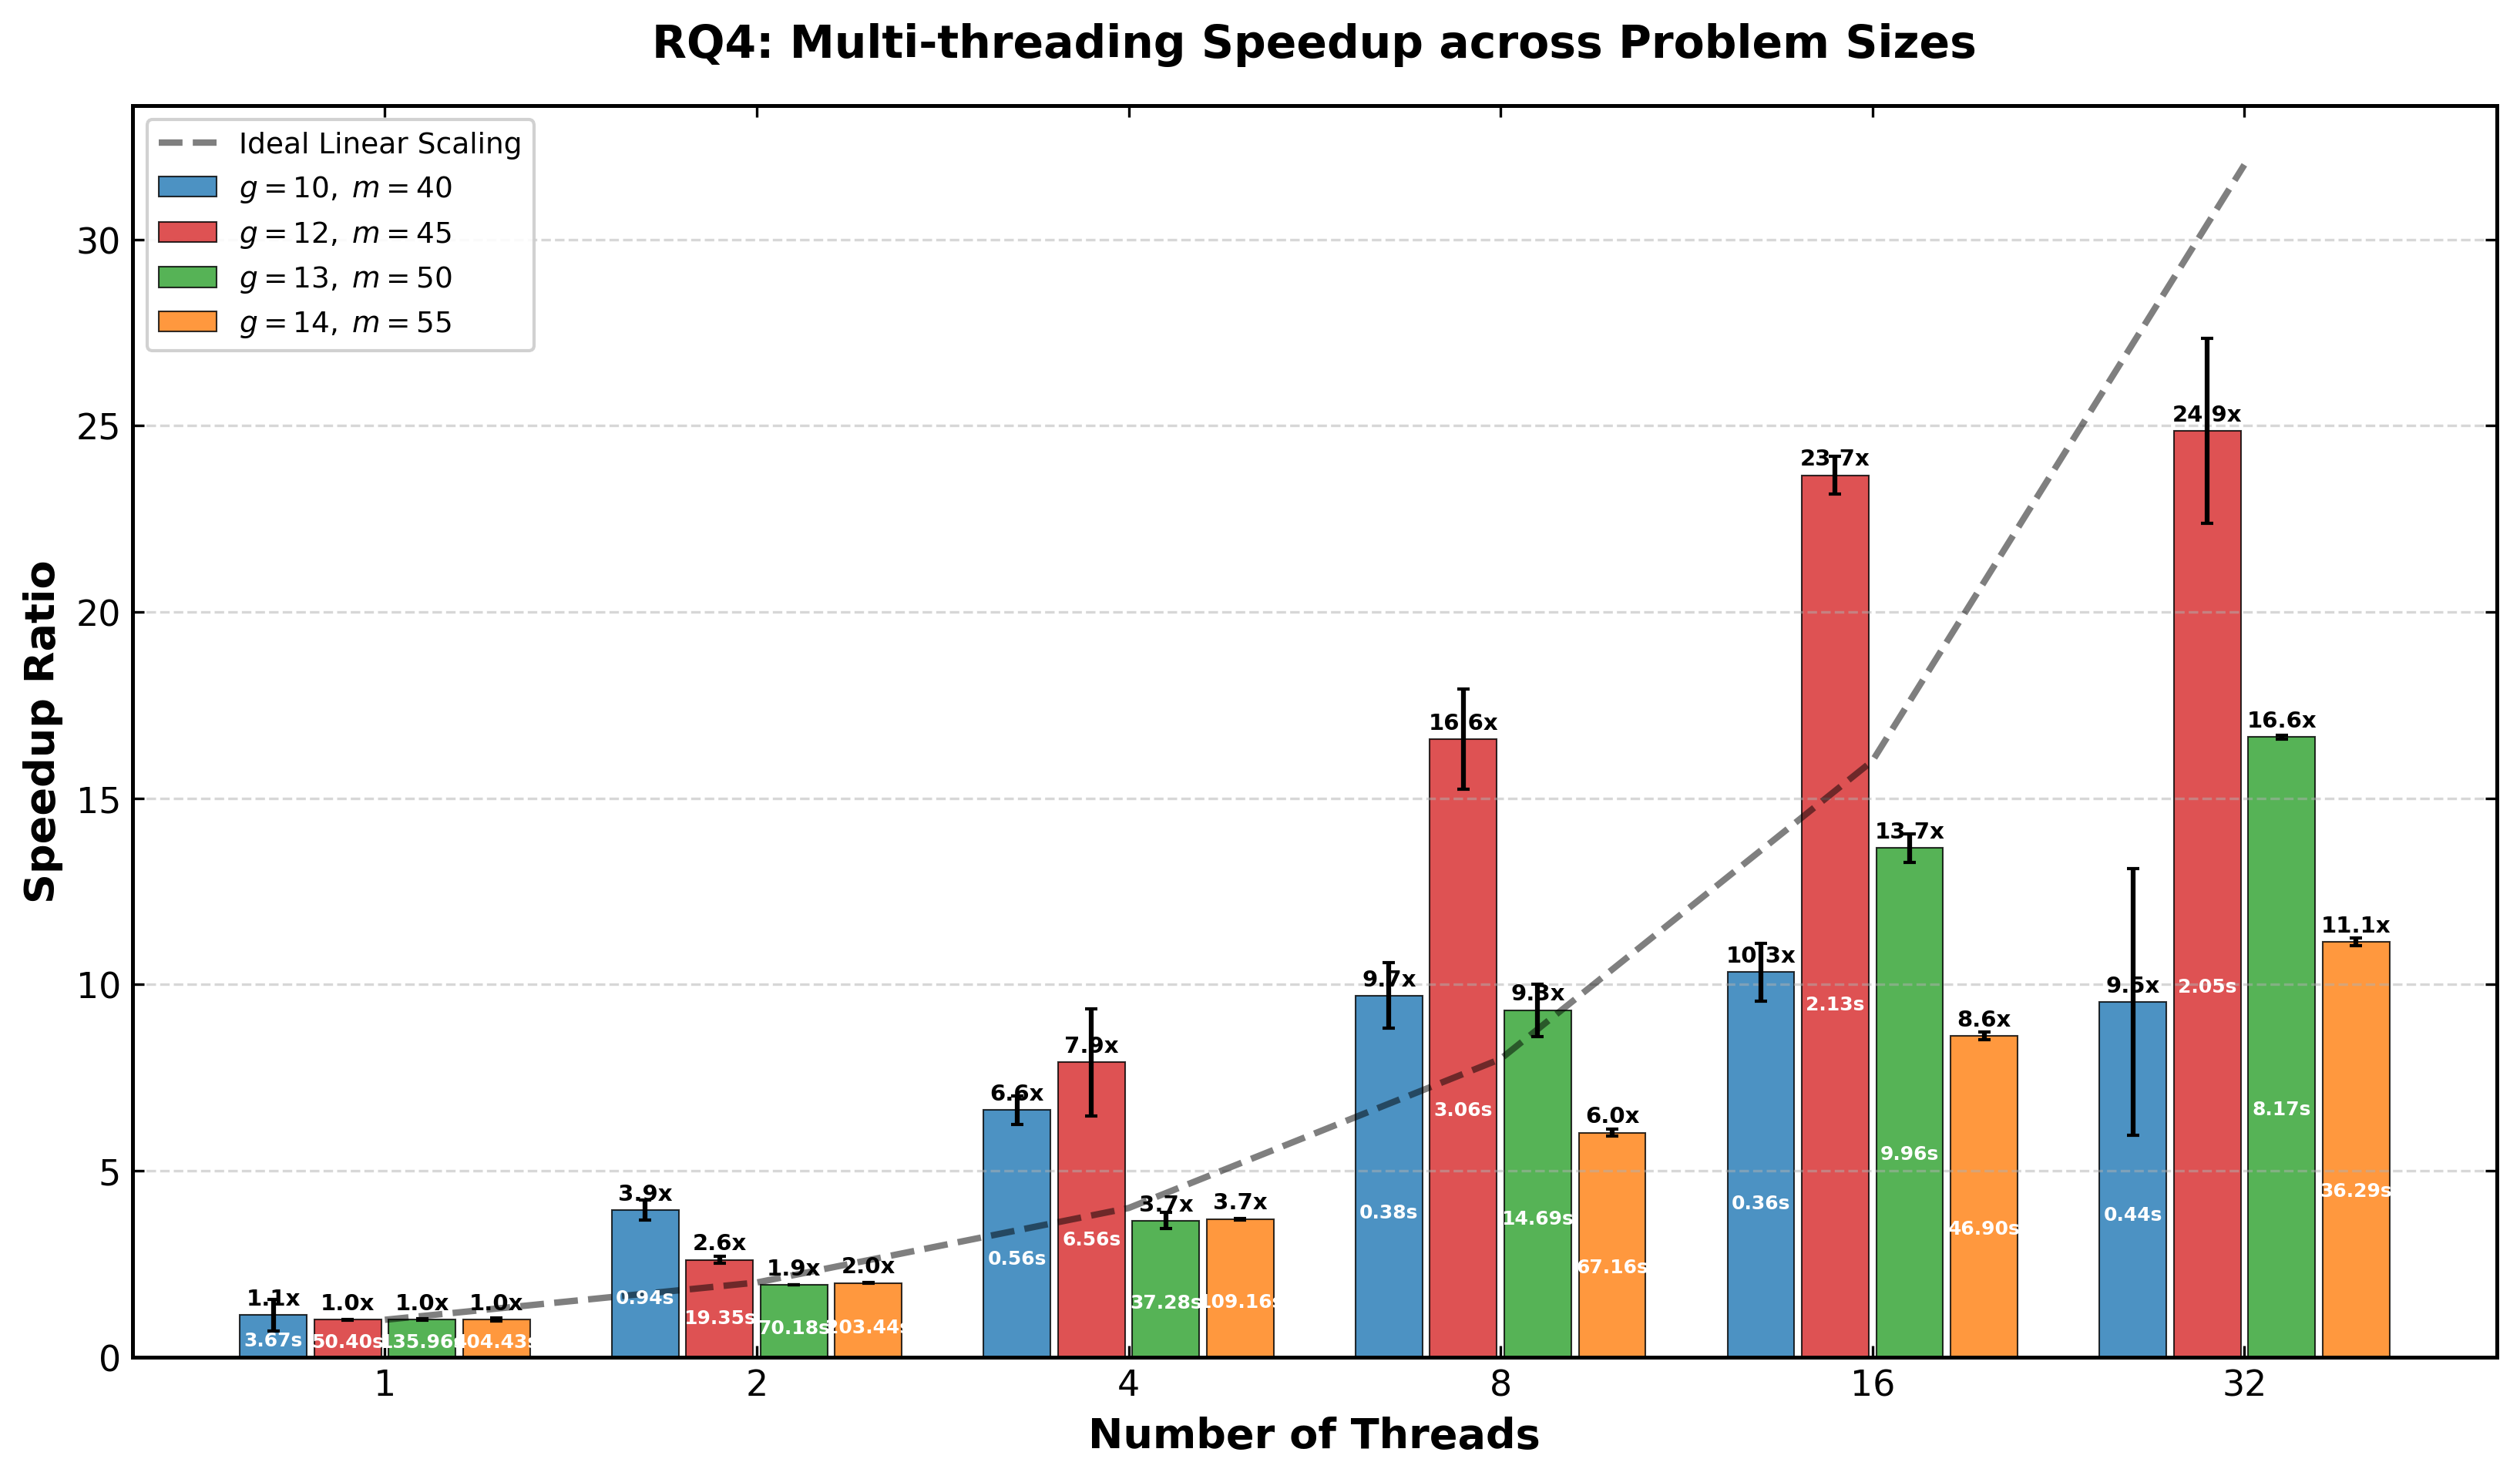
\includegraphics[width=\textwidth]{RQ4_speedup.png}
		\caption{Multi-threading speedup across four problem sizes. Bars show mean speedup with error bars from 3 runs; annotations display both speedup ratio and absolute wall-clock time. The dashed line indicates ideal linear scaling.}
		\label{fig:rq4_speedup_new}
	\end{figure}
	
	\subsubsection{Parallel Efficiency}
	
	Figure~\ref{fig:rq4_efficiency_new} plots the parallel efficiency $E(p) = S(p) / p$. At low thread counts ($p \le 8$), the $g = 10$ and $g = 12$ instances exhibit superlinear efficiency ($E > 1$), with the $g = 10$ instance peaking at $E = 1.96$ at $p = 2$. This arises because each thread's local matrix copy and workspace shrink to fit within the per-core L1/L2 cache when the state space is partitioned: sequential execution must cycle through all $2^g$ states with a single matrix buffer, causing repeated cache evictions, whereas parallel execution keeps each thread's working set cache-resident.
	
	At higher thread counts ($p \ge 16$), efficiency drops below 1.0 for all problem sizes, falling as low as $E = 0.26$ for $g = 10$ at $p = 32$. This degradation has two contributing factors: the per-thread workload becomes too small to amortize synchronization overhead, and the FWHT decoding phase (which remains sequential) becomes a proportionally larger fraction of total runtime.
	
	\begin{figure}[H]
		\centering
		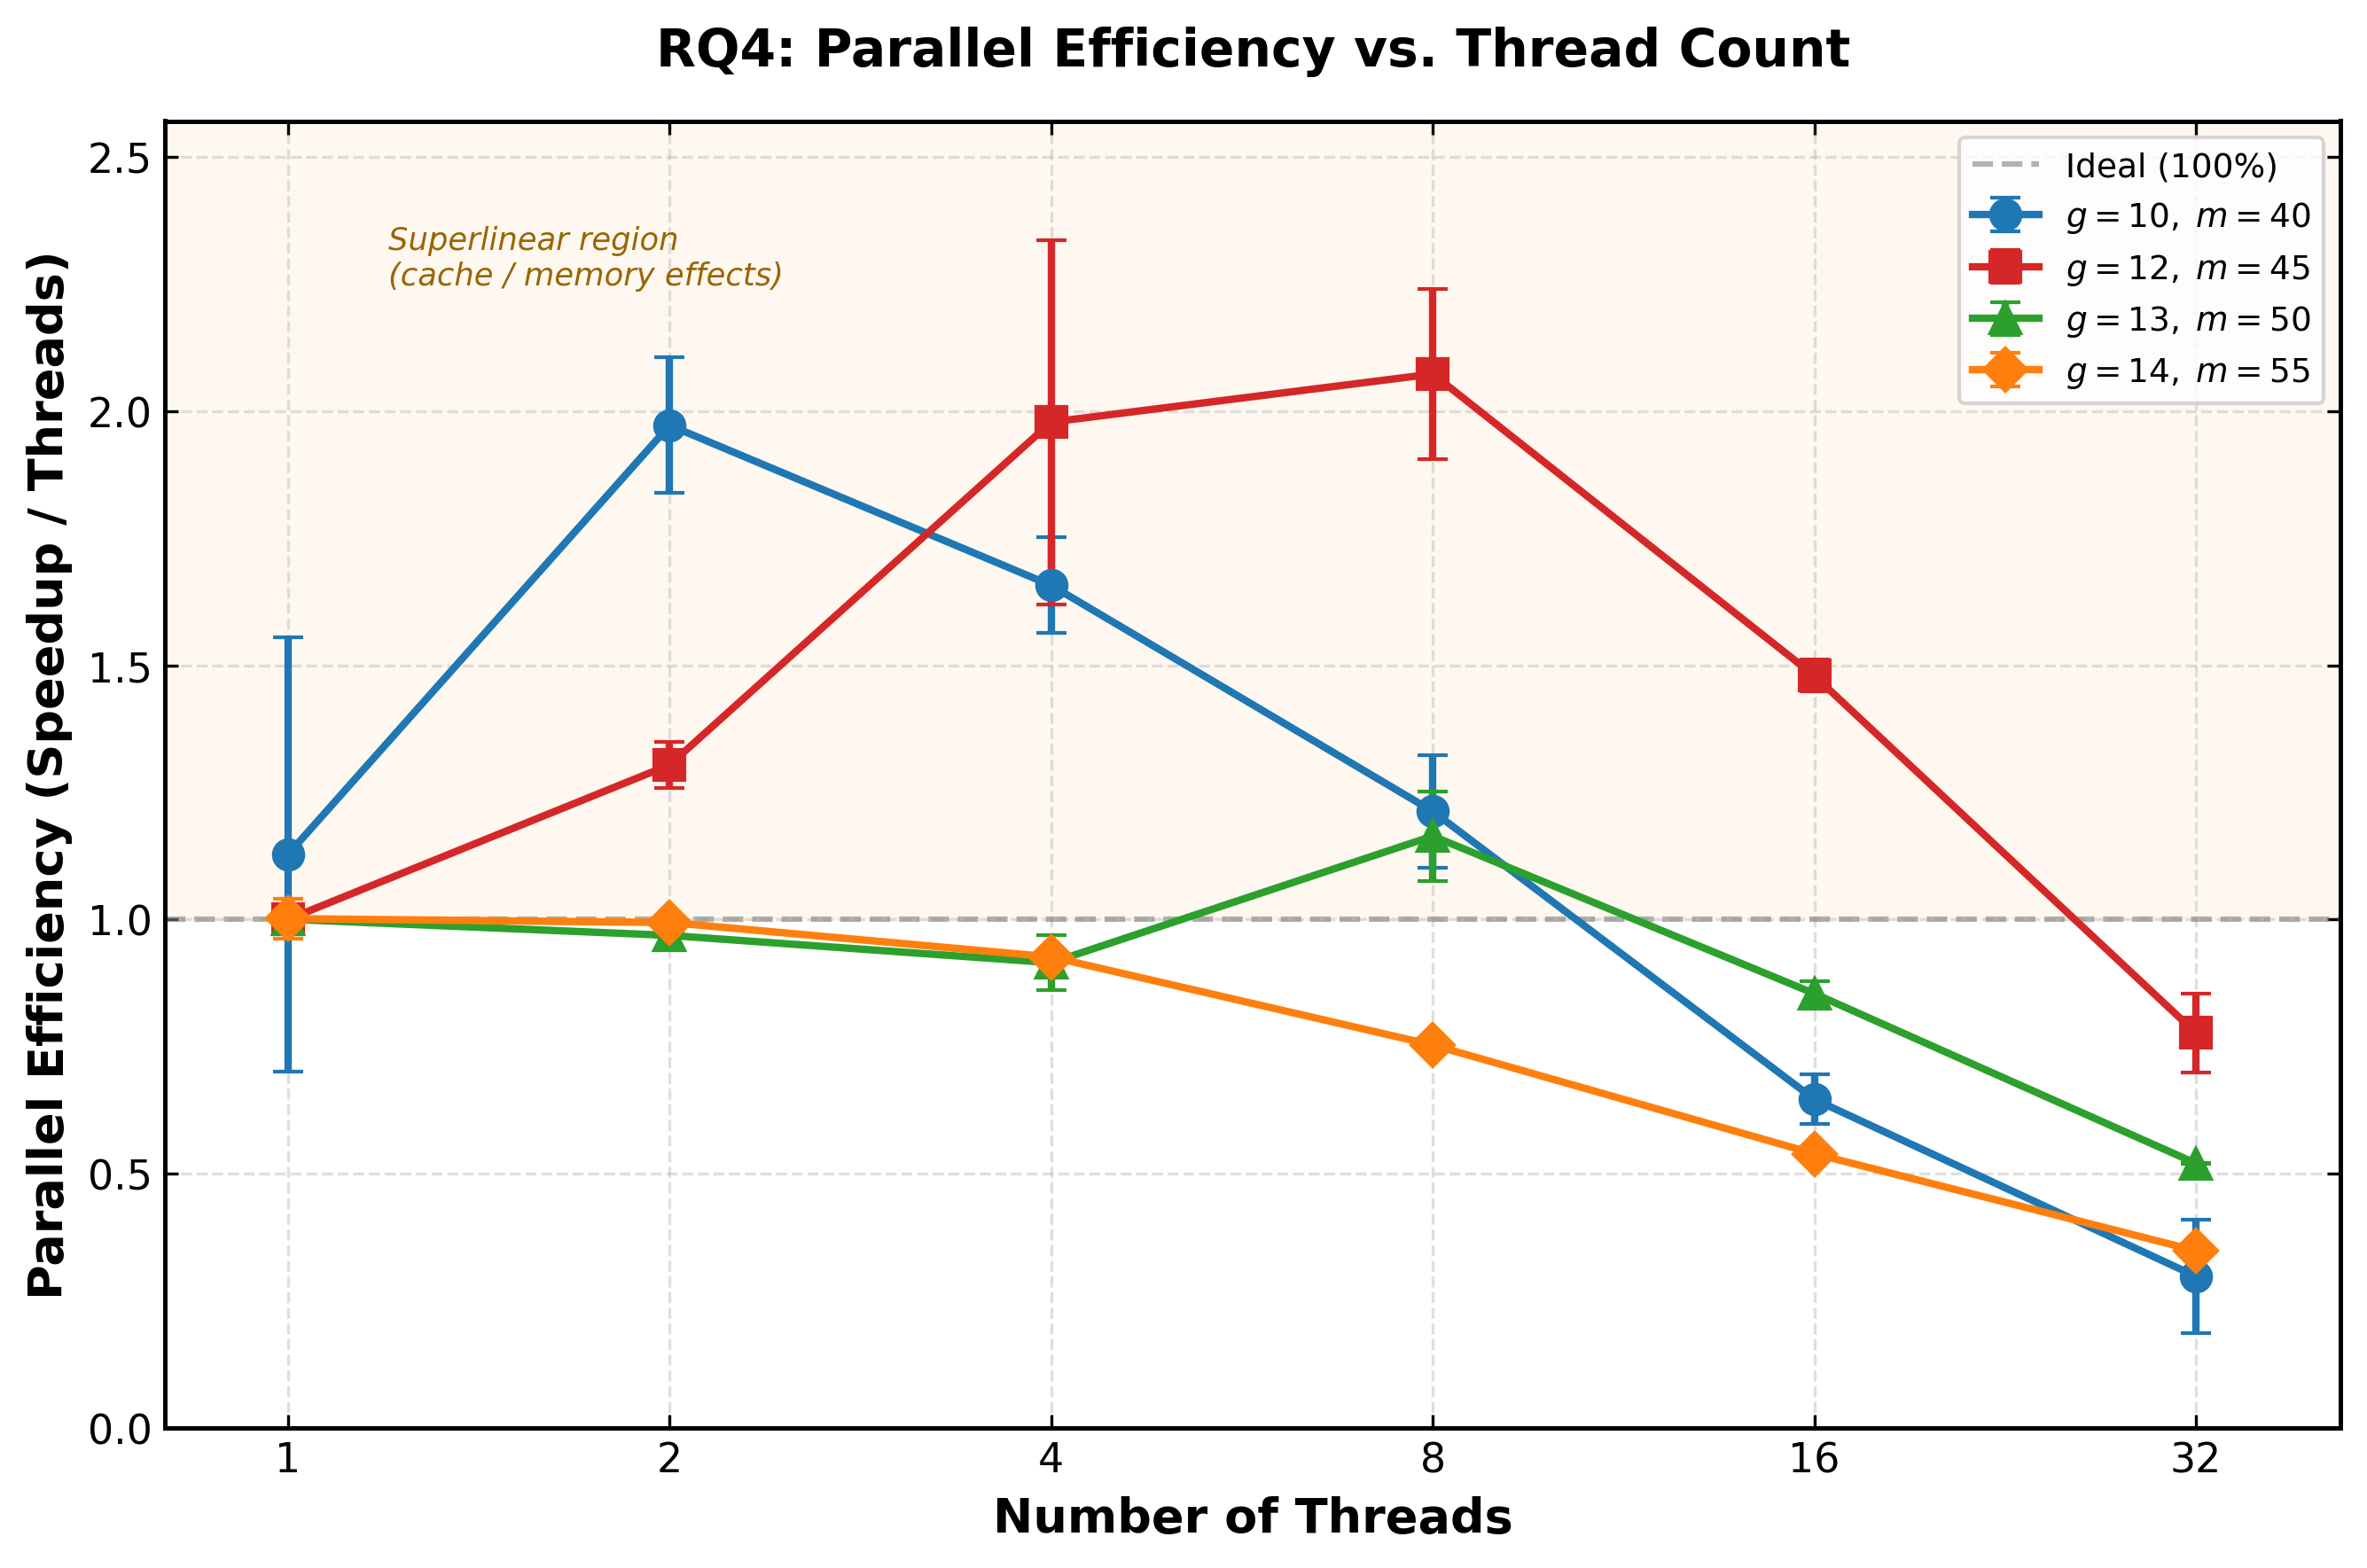
\includegraphics[width=0.82\textwidth]{RQ4_efficiency.png}
		\caption{Parallel efficiency vs.\ thread count. The dashed gray line marks ideal efficiency (100\%). The shaded region above the ideal line indicates superlinear behavior attributed to cache effects.}
		\label{fig:rq4_efficiency_new}
	\end{figure}
	
	\subsubsection{Amdahl's Law Analysis}
	
	To quantify the serial bottleneck, we fit the measured speedup curves to Amdahl's model $S(p) = 1 / (f + (1-f)/p)$, where $f$ is the serial fraction, using a least-squares grid search. Figure~\ref{fig:rq4_amdahl_new} overlays the fitted curves on the measured data.
	
	The fitted serial fractions reveal a clear trend: $f = 0.005$ for $g = 12$, $f = 0.026$ for $g = 13$, and $f = 0.059$ for $g = 14$. This ordering is consistent with the algorithm's structure. The serial components---spanning tree construction, FWHT decoding, and the final normalization---have cost $\bigO(m^2 + g \cdot 2^g)$, which is independent of thread count. As $g$ increases, the parallelizable portion ($2^g$ matrix exponentiations) grows exponentially while the serial overhead grows only polynomially, so the serial fraction $f$ should decrease with~$g$. The data confirms this: the $g = 12$ instance has a negligible serial fraction ($f = 0.005$), predicting a theoretical maximum speedup of $1/f = 200\times$ with unlimited threads.
	
	The $g = 10$ instance deviates from this trend because its total workload ($T_1 = 3.67$\,s) is small enough that fixed-cost overheads---OpenMP thread pool initialization, barrier synchronization, and OS scheduling jitter---inflate the effective serial fraction beyond what the algorithm structure alone would predict.
	
	\begin{figure}[H]
		\centering
		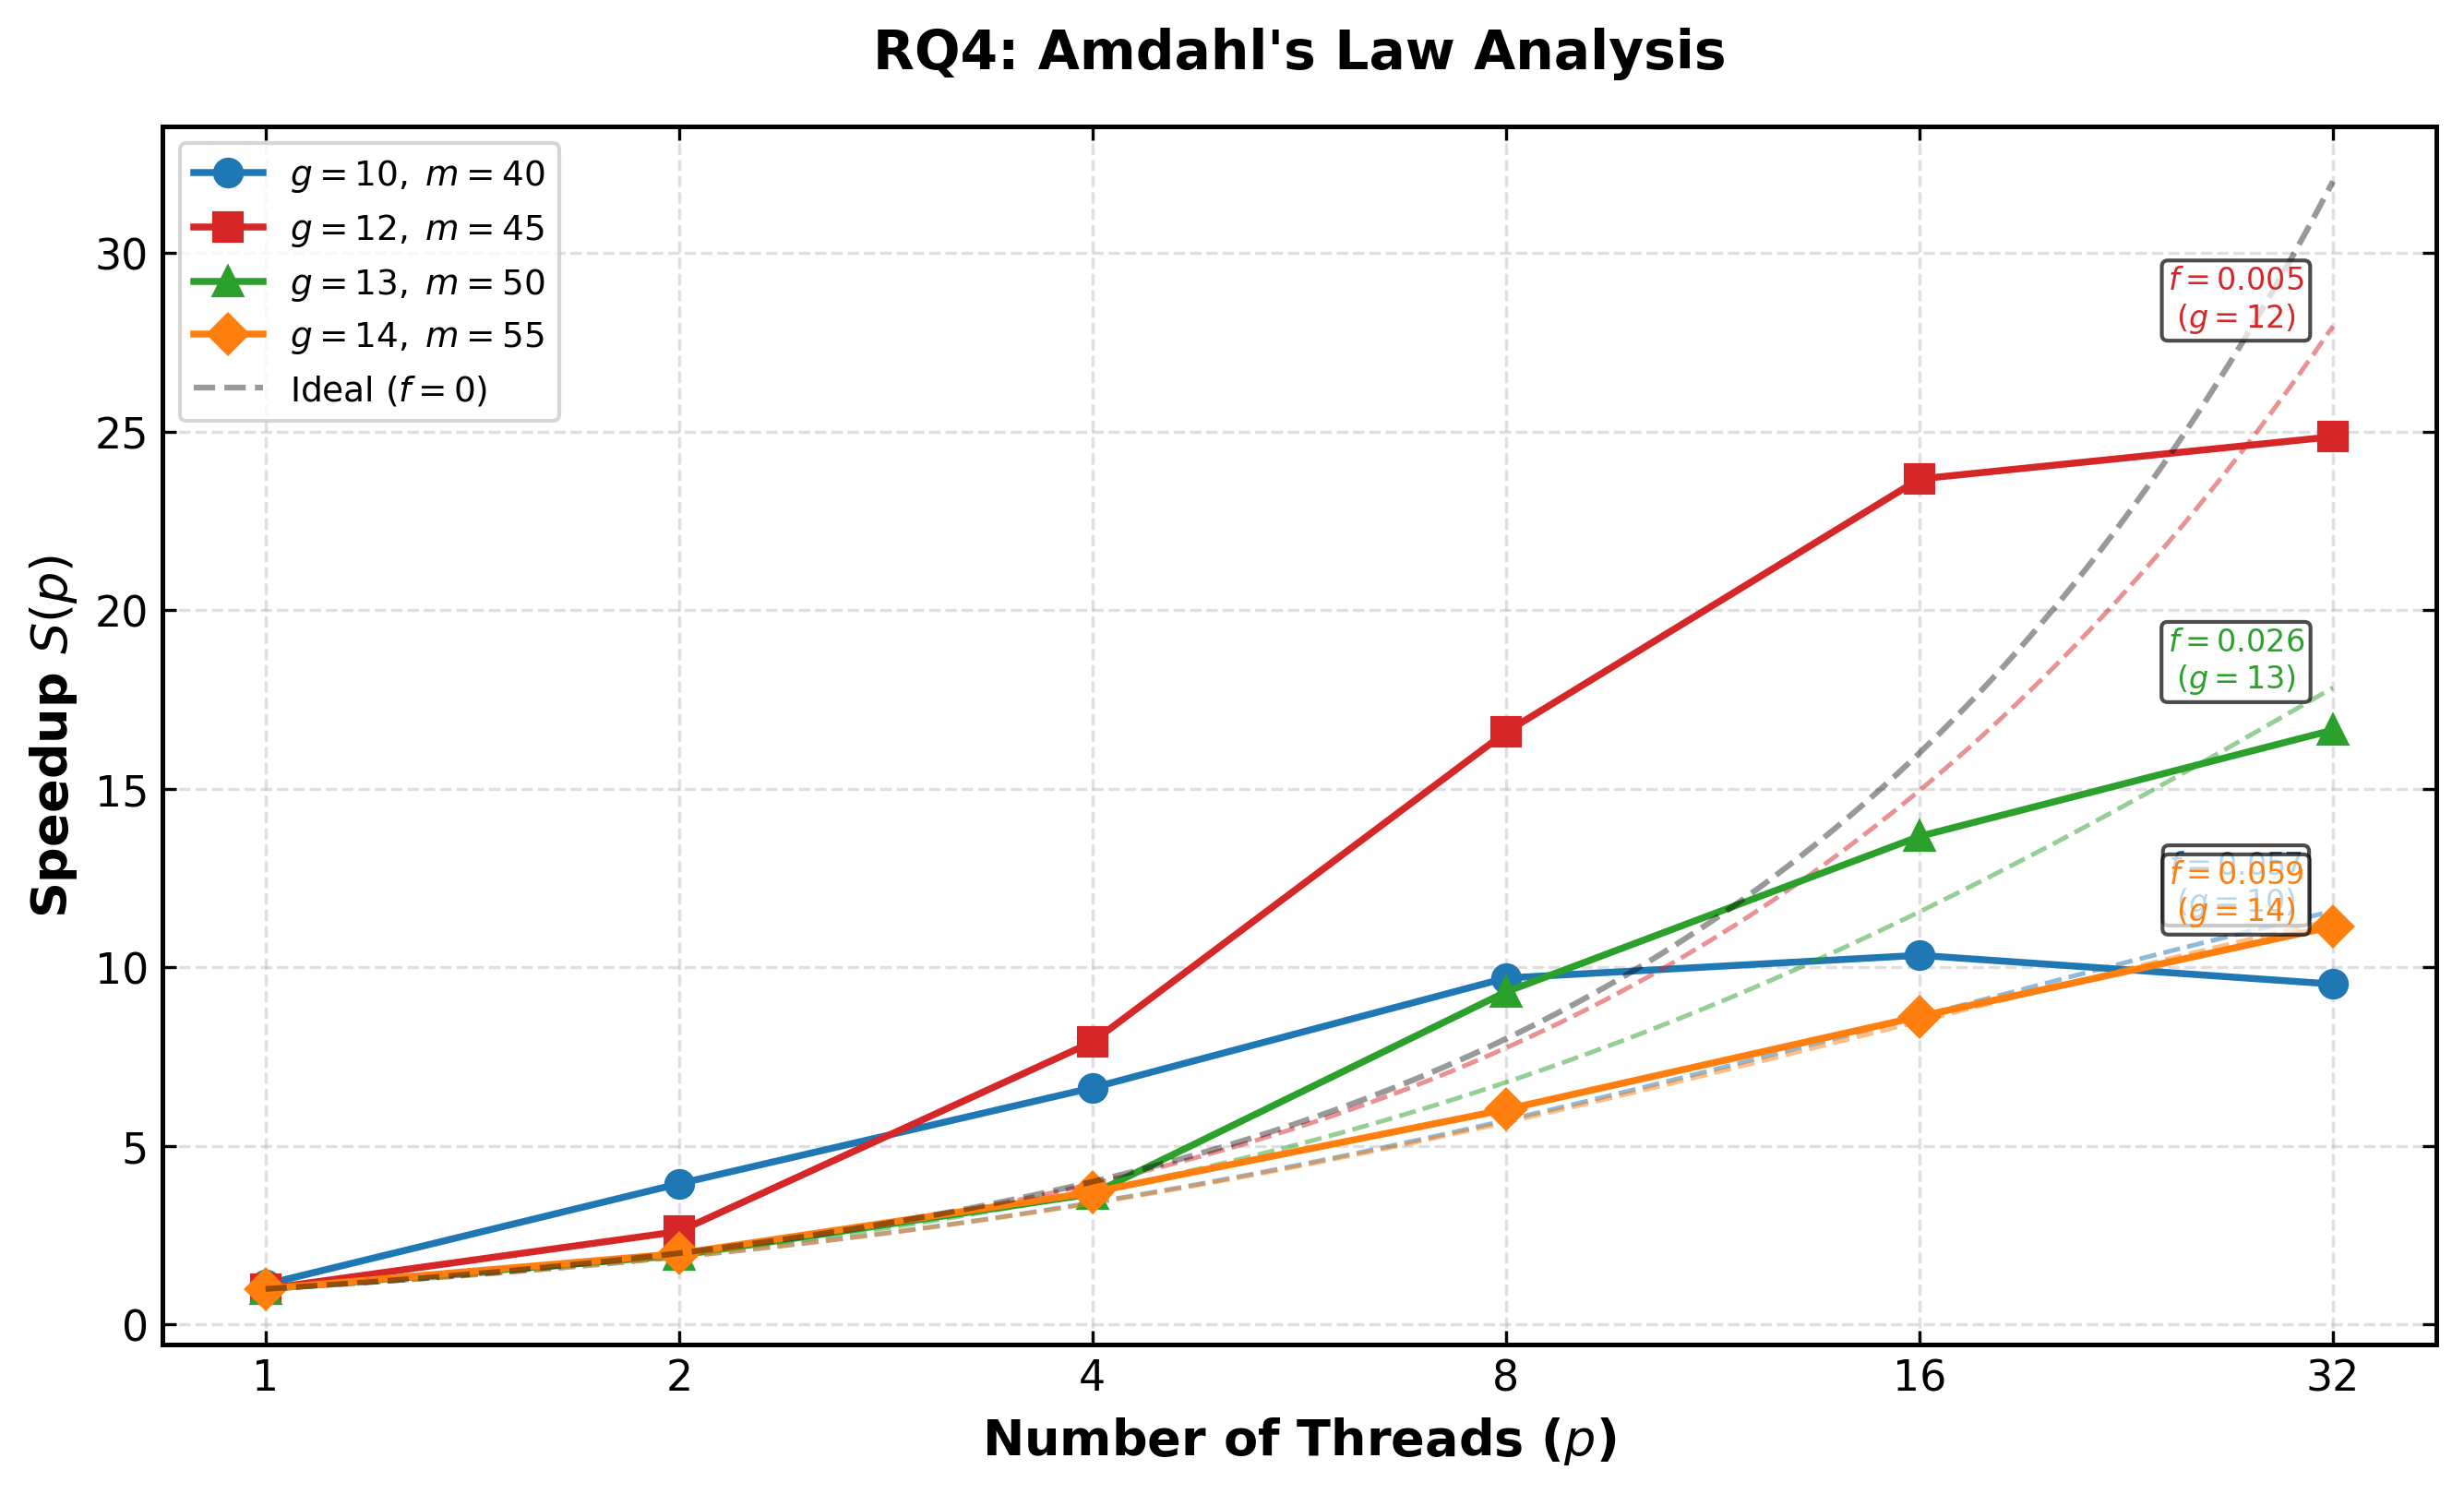
\includegraphics[width=0.82\textwidth]{RQ4_amdahl.png}
		\caption{Amdahl's law fit for each problem size. Solid lines show measured speedup; dashed lines show the fitted Amdahl model with estimated serial fraction $f$. The gray dashed line indicates ideal scaling ($f = 0$).}
		\label{fig:rq4_amdahl_new}
	\end{figure}
	
	\subsubsection{Summary}
	
	Table~\ref{tab:rq4_data_new} presents the complete experimental data.
	
	\begin{table}[H]
		\centering
		\caption{Execution time, speedup, and parallel efficiency across thread counts for four problem sizes. Bold entries indicate the peak speedup for each problem size.}
		\label{tab:rq4_data_new}
		\resizebox{\textwidth}{!}{%
			\begin{tabular}{@{}cl rrrr rrrr@{}}
				\toprule
				& & \multicolumn{4}{c}{\textbf{Time (s)}} & \multicolumn{4}{c}{\textbf{Speedup ($\times$)}} \\
				\cmidrule(lr){3-6} \cmidrule(lr){7-10}
				\textbf{Threads} & & $g\!=\!10$ & $g\!=\!12$ & $g\!=\!13$ & $g\!=\!14$ & $g\!=\!10$ & $g\!=\!12$ & $g\!=\!13$ & $g\!=\!14$ \\
				\midrule
				1  & & 3.67  & 50.40  & 135.96 & 404.43 & 1.0  & 1.0  & 1.0  & 1.0  \\
				2  & & 0.94  & 19.35  & 70.18  & 203.44 & 3.9  & 2.6  & 1.9  & 2.0  \\
				4  & & 0.56  & 6.56   & 37.28  & 109.16 & 6.6  & 7.7  & 3.6  & 3.7  \\
				8  & & 0.38  & 3.06   & 14.69  & 67.16  & 9.6  & 16.5 & 9.3  & 6.0  \\
				16 & & 0.36  & 2.13   & 9.96   & 46.90  & \textbf{10.3} & 23.7 & 13.7 & 8.6  \\
				32 & & 0.44  & 2.05   & 8.17   & 36.29  & 8.4  & \textbf{24.9} & \textbf{16.6} & \textbf{11.1} \\
				\midrule
				\multicolumn{2}{l}{Amdahl $f$} & ---   & 0.005  & 0.026  & 0.059  & & & & \\
				\bottomrule
			\end{tabular}%
		}
	\end{table}
	
	The RQ4 results demonstrate that the parallelization of the $2^g$ state evaluations is effective, with the best case ($g = 12$) reaching $24.9\times$ on 32 threads. The scaling behavior depends non-trivially on problem size: moderate-sized instances benefit from superlinear cache effects, while larger instances are constrained by memory bandwidth, and very small instances are limited by synchronization overhead. The Amdahl's law analysis confirms that the serial fraction decreases with circuit rank, suggesting that the algorithm's parallelism becomes more efficient as the problem grows---a desirable property for scaling to harder instances.
	
	\subsection{RQ5: Evaluation on Real-World Graphs}
	\label{subsec:rq5}

	To validate the crossover observed on synthetic instances, we evaluated both solvers on real-world graphs from two application domains.

	\textbf{Datasets.} We selected 45 molecular graphs from three TUDatasets~\cite{TUDatasets}: MUTAG (mutagenicity, 15 graphs, $g = 4$--$11$), AIDS (molecular compounds, 15 graphs, $g = 3$--$10$), and PTC\_MR (carcinogenicity, 15 graphs, $g = 3$--$10$). We also extracted 16 subgraphs from two infrastructure networks in the Network Data Repository~\cite{NetworkRepository}: the US Western States power grid (8 subgraphs, $g = 7$--$16$) and the European road network (8 subgraphs, $g = 10$--$18$). All graphs were preprocessed to satisfy the Eulerian condition by adding a minimum set of edges to make all vertex degrees even. This augmentation is necessary because Eulerian circuits only exist in graphs where every vertex has even degree; the added edges increase the circuit rank by at most the number of edges added, and we verified that the resulting circuit ranks remain representative of the original graph complexity. Importantly, the FWHT runtime depends only on $g$ and $m$, so the augmentation affects the problem size but not the algorithmic properties being evaluated.

	\textbf{Molecular graphs.} Table~\ref{tab:rq5_molecular} summarizes the molecular results. All 45 graphs have circuit rank at most~11, placing them firmly in the DFS-favorable regime identified in RQ2. The FWHT solver completes all instances in under 0.23\,s, but DFS is consistently 14--$8500\times$ faster, confirming that the algebraic approach provides no speedup when $g$ is small.

	\begin{table}[H]
		\centering
		\caption{RQ5: Molecular graph results (DFS-favorable regime).}
		\label{tab:rq5_molecular}
		\begin{tabular}{lcccc}
			\toprule
			Dataset & Graphs & $g$ range & FWHT time (s) & DFS time (s) \\
			\midrule
			MUTAG   & 15 & 4--11 & 0.060--0.222 & $7 \times 10^{-6}$--$4.7 \times 10^{-3}$ \\
			AIDS    & 15 & 3--10 & 0.049--0.142 & $6 \times 10^{-6}$--$4.8 \times 10^{-3}$ \\
			PTC\_MR & 15 & 3--10 & 0.049--0.164 & $5 \times 10^{-6}$--$1.4 \times 10^{-3}$ \\
			\bottomrule
		\end{tabular}
	\end{table}

	\textbf{Infrastructure graphs.} Table~\ref{tab:rq5_infra} reports the detailed comparison on infrastructure subgraphs, sorted by circuit rank. The crossover is clearly visible: for $g \le 11$, DFS completes in under 100\,ms and outperforms FWHT by $4$--$18\times$; at $g = 12$, the methods are comparable, with speedup ranging from $1.1\times$ to $23\times$ depending on graph density; for $g \ge 14$, FWHT is consistently faster, reaching $177\times$ on a power grid subgraph with $g = 14$. At $g = 16$ and $g = 18$, DFS fails to complete within the 600\,s timeout on two instances, while FWHT solves all 16 instances, including the largest ($g = 18$, $m = 50$) in 49.9\,s.

	\begin{table}[H]
		\centering
		\caption{RQ5: Infrastructure graph comparison (sorted by circuit rank $g$). Speedup $= t_{\text{DFS}} / t_{\text{FWHT}}$; values ${>}1$ favor FWHT. TO\,=\,timeout at 600\,s.}
		\label{tab:rq5_infra}
		\resizebox{\textwidth}{!}{%
			\begin{tabular}{lrrrrrr}
				\toprule
				Graph & $n$ & $m$ & $g$ & FWHT (s) & DFS (s) & Speedup \\
				\midrule
				power-6   & 13 & 19 & 7  & 0.09  & 0.003   & $0.03\times$ \\
				power-2   & 15 & 23 & 9  & 0.12  & 0.10    & $0.82\times$ \\
				road-1    & 22 & 31 & 10 & 0.18  & 0.01    & $0.06\times$ \\
				road-4    & 22 & 32 & 11 & 0.22  & 0.04    & $0.20\times$ \\
				road-2    & 25 & 35 & 11 & 0.24  & 0.06    & $0.26\times$ \\
				\midrule
				power-4   & 15 & 26 & 12 & 0.25  & 5.81    & $\mathbf{23\times}$ \\
				road-5    & 25 & 36 & 12 & 0.40  & 0.75    & $1.9\times$ \\
				road-6    & 25 & 36 & 12 & 0.40  & 0.45    & $1.1\times$ \\
				\midrule
				power-5   & 15 & 28 & 14 & 0.76  & 134     & $\mathbf{177\times}$ \\
				power-7   & 14 & 27 & 14 & 0.72  & 19.6    & $27\times$ \\
				road-7    & 28 & 41 & 14 & 1.89  & 3.53    & $1.9\times$ \\
				road-0    & 26 & 40 & 15 & 3.32  & 15.4    & $4.6\times$ \\
				power-1   & 29 & 43 & 15 & 4.45  & 152     & $34\times$ \\
				power-3   & 29 & 44 & 16 & 10.2  & 199     & $20\times$ \\
				power-0   & 21 & 36 & 16 & 4.83  & TO      & ${>}124\times$ \\
				road-3    & 33 & 50 & 18 & 49.9  & TO      & ${>}12\times$ \\
				\bottomrule
			\end{tabular}%
		}
	\end{table}

	The crossover at $g \approx 12$ is consistent with the synthetic experiments in RQ2. Notably, the variation in speedup at the same circuit rank (e.g., $1.1\times$ to $23\times$ at $g = 12$) reflects the density dependence identified in RQ2: power grid subgraphs, which are denser relative to their vertex count, have exponentially more Eulerian circuits, making DFS slower while FWHT runtime remains structure-agnostic. These results confirm that the crossover observed on synthetic benchmarks generalizes to naturally occurring graph structures.

	\section{Discussion and Limitations}
	\label{sec:discussion}
	
	\textbf{Scope of applicability.} The $\bigO(2^g)$ exponential dependence strictly limits the algorithm to graphs with moderate circuit rank. For dense graphs where $g = \Theta(m)$, backtracking or approximation methods remain more appropriate. Our experimental evaluation (RQ2) shows that even within the tractable regime, the crossover point between FWHT and DFS depends on graph density: the method is most advantageous for dense graphs at moderate circuit rank, while very sparse graphs at low circuit rank are better served by DFS.
	
	\textbf{Strength of the DFS baseline.} We also implemented a bridge-pruned DFS variant incorporating Fleury's rule via Tarjan's algorithm. On all 59 completed instances, the bridge-pruned variant produced identical raw trail counts as the naive baseline, indicating that the DFS search tree contains no dead-end branches caused by bridge traversals for these graph families. Moreover, the per-step $\bigO(n{+}m)$ bridge-detection overhead made the pruned variant $1.2$--$2.2\times$ slower than the naive baseline. The speedups reported in Tables~\ref{tab:rq5_infra} therefore use the faster naive DFS, providing a conservative (i.e., less favorable to FWHT) comparison. This finding suggests that the crossover analysis is robust: standard algorithmic improvements to the DFS baseline do not shift the crossover point, because the bottleneck is the exponential growth of valid Euler circuits rather than dead-end exploration.
	
	\textbf{Correctness verification.} We verified the implementation against brute-force enumeration on all graphs with $g \le 8$ in our test suite. For the 59 real-world instances where DFS completed (out of 61; two timed out at $g = 16$ and $g = 18$), the FWHT and DFS circuit counts agree exactly: the raw DFS trail count satisfies $\text{raw} = \ec(G) \cdot d(v_0)$ in every case. This cross-validation across two independent algorithmic paradigms---algebraic (FWHT) and combinatorial (backtracking)---provides strong evidence of correctness for $g$ up to~16. For larger~$g$ where DFS becomes infeasible, independent verification via MCMC estimates~\cite{CreedGoldberg2013} or combinatorial identities for specific graph families remains an important direction.
	
	\textbf{Real-world validation.} Our evaluation on 61 real-world graphs from molecular chemistry and infrastructure networks (RQ5) confirms that the crossover at $g \approx 12$ observed on synthetic benchmarks generalizes to naturally occurring graph structures. The molecular graphs all lie in the DFS-favorable regime ($g \le 11$), while infrastructure subgraphs span the crossover region and demonstrate FWHT speedups exceeding $100\times$ at $g \ge 14$. We note that the Eulerian augmentation preprocessing increases the circuit rank; developing augmentation strategies that minimize this increase is an interesting direction.
	
	\textbf{Structure-agnostic runtime, structure-sensitive output.} A recurring theme across our experiments is the separation between computational cost and combinatorial output. The FWHT runtime depends only on $g$ and $m$, not on graph topology (RQ2, RQ3), whereas the number of Eulerian circuits varies by orders of magnitude across graph families at the same $(g, m)$. This decoupling is a fundamental property of the algebraic approach: the trace formula evaluates the count via a fixed number of matrix operations, independent of the output size.
	
	\textbf{Parallelization.} The independent per-state construction eliminates inter-thread communication, and the RQ4 results show effective speedup for problems with sufficient per-thread workload. The primary bottleneck to further scaling is the sequential FWHT decoding phase, whose cost $\bigO(g \cdot 2^g)$ is negligible for moderate $g$ but becomes relevant as $g$ grows.
	
	\section{Conclusion}
	\label{sec:conclusion}
	We have described an efficient implementation of the Luo homological trace formula~\cite{Luo2025} for exact Eulerian circuit counting in undirected graphs, leveraging the Fourier-transform structure identified by Luo and Roy~\cite{LR24} to enable FWHT-based spectral decoding. By combining this with independent per-state matrix construction and OpenMP parallelization, the implementation achieves practical performance for graphs with small circuit rank. Rigorous complexity analysis establishes the $\bigO(2^g \cdot m^3 \log m)$ time bound with formal proofs for each component, and the FPT classification follows as a corollary.
	
	Experimental results on synthetic and real-world graphs provide four key findings. First, the crossover between FWHT and backtracking is density-dependent: the algebraic method becomes competitive at $g \approx 10$--$12$ for dense graphs (as measured against an unoptimized DFS baseline), while sparse graphs remain DFS-favorable at low circuit rank. Second, this crossover generalizes to real-world graphs from molecular chemistry and infrastructure networks, with FWHT achieving speedups exceeding $100\times$ on infrastructure subgraphs with $g \ge 14$. Third, the runtime scales as $\bigO(m^3 \log m)$ at fixed circuit rank in a structure-agnostic manner, as validated by normalized time analysis across diverse graph families. Fourth, the parallelization achieves near-linear speedup for moderate problem sizes, with Amdahl's law analysis confirming that the serial fraction decreases with circuit rank.
	
	Future directions include: (1) comparison against optimized backtracking implementations with advanced pruning heuristics; (2) exploration of sparse matrix techniques or tensor network methods to reduce the effective base of the exponential; and (3) investigation of whether the homological filtering mechanism can be adapted to yield efficient randomized approximation schemes for high circuit rank graphs.
	\section*{Code and Data Availability}
	The C++ implementation, graph generators, and all experimental data are available at \url{https://github.com/AndyShan11/FWHT-Counting-Eulerian-Circuits}. The repository includes build instructions, scripts to reproduce all figures and tables, and the raw timing data.

\bibliographystyle{ACM-Reference-Format}
\bibliography{references}

\end{document}